% Options for packages loaded elsewhere
\PassOptionsToPackage{unicode}{hyperref}
\PassOptionsToPackage{hyphens}{url}
%
\documentclass[
  11pt,
]{article}
\usepackage{amsmath,amssymb}
\usepackage{iftex}
\ifPDFTeX
  \usepackage[T1]{fontenc}
  \usepackage[utf8]{inputenc}
  \usepackage{textcomp} % provide euro and other symbols
\else % if luatex or xetex
  \usepackage{unicode-math} % this also loads fontspec
  \defaultfontfeatures{Scale=MatchLowercase}
  \defaultfontfeatures[\rmfamily]{Ligatures=TeX,Scale=1}
\fi
\usepackage{lmodern}
\ifPDFTeX\else
  % xetex/luatex font selection
\fi
% Use upquote if available, for straight quotes in verbatim environments
\IfFileExists{upquote.sty}{\usepackage{upquote}}{}
\IfFileExists{microtype.sty}{% use microtype if available
  \usepackage[]{microtype}
  \UseMicrotypeSet[protrusion]{basicmath} % disable protrusion for tt fonts
}{}
\makeatletter
\@ifundefined{KOMAClassName}{% if non-KOMA class
  \IfFileExists{parskip.sty}{%
    \usepackage{parskip}
  }{% else
    \setlength{\parindent}{0pt}
    \setlength{\parskip}{6pt plus 2pt minus 1pt}}
}{% if KOMA class
  \KOMAoptions{parskip=half}}
\makeatother
\usepackage{xcolor}
\usepackage[margin=1in]{geometry}
\usepackage{color}
\usepackage{fancyvrb}
\newcommand{\VerbBar}{|}
\newcommand{\VERB}{\Verb[commandchars=\\\{\}]}
\DefineVerbatimEnvironment{Highlighting}{Verbatim}{commandchars=\\\{\}}
% Add ',fontsize=\small' for more characters per line
\usepackage{framed}
\definecolor{shadecolor}{RGB}{248,248,248}
\newenvironment{Shaded}{\begin{snugshade}}{\end{snugshade}}
\newcommand{\AlertTok}[1]{\textcolor[rgb]{0.94,0.16,0.16}{#1}}
\newcommand{\AnnotationTok}[1]{\textcolor[rgb]{0.56,0.35,0.01}{\textbf{\textit{#1}}}}
\newcommand{\AttributeTok}[1]{\textcolor[rgb]{0.13,0.29,0.53}{#1}}
\newcommand{\BaseNTok}[1]{\textcolor[rgb]{0.00,0.00,0.81}{#1}}
\newcommand{\BuiltInTok}[1]{#1}
\newcommand{\CharTok}[1]{\textcolor[rgb]{0.31,0.60,0.02}{#1}}
\newcommand{\CommentTok}[1]{\textcolor[rgb]{0.56,0.35,0.01}{\textit{#1}}}
\newcommand{\CommentVarTok}[1]{\textcolor[rgb]{0.56,0.35,0.01}{\textbf{\textit{#1}}}}
\newcommand{\ConstantTok}[1]{\textcolor[rgb]{0.56,0.35,0.01}{#1}}
\newcommand{\ControlFlowTok}[1]{\textcolor[rgb]{0.13,0.29,0.53}{\textbf{#1}}}
\newcommand{\DataTypeTok}[1]{\textcolor[rgb]{0.13,0.29,0.53}{#1}}
\newcommand{\DecValTok}[1]{\textcolor[rgb]{0.00,0.00,0.81}{#1}}
\newcommand{\DocumentationTok}[1]{\textcolor[rgb]{0.56,0.35,0.01}{\textbf{\textit{#1}}}}
\newcommand{\ErrorTok}[1]{\textcolor[rgb]{0.64,0.00,0.00}{\textbf{#1}}}
\newcommand{\ExtensionTok}[1]{#1}
\newcommand{\FloatTok}[1]{\textcolor[rgb]{0.00,0.00,0.81}{#1}}
\newcommand{\FunctionTok}[1]{\textcolor[rgb]{0.13,0.29,0.53}{\textbf{#1}}}
\newcommand{\ImportTok}[1]{#1}
\newcommand{\InformationTok}[1]{\textcolor[rgb]{0.56,0.35,0.01}{\textbf{\textit{#1}}}}
\newcommand{\KeywordTok}[1]{\textcolor[rgb]{0.13,0.29,0.53}{\textbf{#1}}}
\newcommand{\NormalTok}[1]{#1}
\newcommand{\OperatorTok}[1]{\textcolor[rgb]{0.81,0.36,0.00}{\textbf{#1}}}
\newcommand{\OtherTok}[1]{\textcolor[rgb]{0.56,0.35,0.01}{#1}}
\newcommand{\PreprocessorTok}[1]{\textcolor[rgb]{0.56,0.35,0.01}{\textit{#1}}}
\newcommand{\RegionMarkerTok}[1]{#1}
\newcommand{\SpecialCharTok}[1]{\textcolor[rgb]{0.81,0.36,0.00}{\textbf{#1}}}
\newcommand{\SpecialStringTok}[1]{\textcolor[rgb]{0.31,0.60,0.02}{#1}}
\newcommand{\StringTok}[1]{\textcolor[rgb]{0.31,0.60,0.02}{#1}}
\newcommand{\VariableTok}[1]{\textcolor[rgb]{0.00,0.00,0.00}{#1}}
\newcommand{\VerbatimStringTok}[1]{\textcolor[rgb]{0.31,0.60,0.02}{#1}}
\newcommand{\WarningTok}[1]{\textcolor[rgb]{0.56,0.35,0.01}{\textbf{\textit{#1}}}}
\usepackage{graphicx}
\makeatletter
\def\maxwidth{\ifdim\Gin@nat@width>\linewidth\linewidth\else\Gin@nat@width\fi}
\def\maxheight{\ifdim\Gin@nat@height>\textheight\textheight\else\Gin@nat@height\fi}
\makeatother
% Scale images if necessary, so that they will not overflow the page
% margins by default, and it is still possible to overwrite the defaults
% using explicit options in \includegraphics[width, height, ...]{}
\setkeys{Gin}{width=\maxwidth,height=\maxheight,keepaspectratio}
% Set default figure placement to htbp
\makeatletter
\def\fps@figure{htbp}
\makeatother
\setlength{\emergencystretch}{3em} % prevent overfull lines
\providecommand{\tightlist}{%
  \setlength{\itemsep}{0pt}\setlength{\parskip}{0pt}}
\setcounter{secnumdepth}{-\maxdimen} % remove section numbering
\usepackage{amsmath}
\usepackage{amssymb}
\usepackage{mathtools}
\usepackage{enumitem}
\usepackage{setspace}
\usepackage{amsthm}
\usepackage{centernot}
\DeclareMathOperator\arctanh{arctanh}
\DeclareMathOperator{\Unif}{Unif}
\DeclareMathOperator{\Var}{Var}
\DeclareMathOperator{\Cov}{Cov}
\DeclareMathOperator{\Bern}{Bernoulli}
\DeclareMathOperator{\Bin}{Bin}
\DeclareMathOperator{\Pois}{Poisson}
\newtheorem{theorem}{Theorem}[section]
\newtheorem{definition}{Definition}[section]
\newtheorem{fact}{Fact}[section]
\newtheorem{prop}{Proposition}[section]
\newtheorem{corollary}{Corollary}[section]
\newtheorem{lemma}{Lemma}[section]
\newcommand{\iid}[0]{\overset{\mathrm{iid}}{\sim}}
\ifLuaTeX
  \usepackage{selnolig}  % disable illegal ligatures
\fi
\IfFileExists{bookmark.sty}{\usepackage{bookmark}}{\usepackage{hyperref}}
\IfFileExists{xurl.sty}{\usepackage{xurl}}{} % add URL line breaks if available
\urlstyle{same}
\hypersetup{
  pdftitle={Regression Analysis Examples in R},
  hidelinks,
  pdfcreator={LaTeX via pandoc}}

\title{Regression Analysis Examples in R}
\author{}
\date{\vspace{-2.5em}}

\begin{document}
\maketitle

\section{Chapter 2 - Simple Linear
Regression}\label{chapter-2---simple-linear-regression}

\subsection{Example. Airfreight Data}\label{example.-airfreight-data}

\begin{center}
    \begin{tabular}{|c|c|c|c|c|c|c|c|c|c|c|}
        \hline
        & 1 & 2 & 3 & 4 & 5 & 6 & 7 & 8 & 9 & 10\\
        \hline
        Shipment Route ($x$) & 1 & 0 & 2 & 0 & 3 & 1 & 0 & 1 & 2 & 0\\
        Airfreight Breakage ($y$) & 16 & 9 & 17 & 12 & 22 & 13 & 8 & 15 & 19 & 11\\
        \hline
    \end{tabular}
\end{center}

\begin{enumerate}
\def\labelenumi{\alph{enumi})}
\tightlist
\item
  Compute the ANOVA table
\item
  Compute the confidence intervals for the parameters
\item
  Compute the confidence interval on the average (mean) response when
  \(X = 1\).
\item
  What is the total variability in \(y\) explained by this model?
\end{enumerate}

\subsection{Solution.}\label{solution.}

\subsubsection{Part a.}\label{part-a.}

We can compute the anova table manually as follows,

\[S_{xx} = \sum_{i=1}^n (x_i-\bar{x})^2 = \sum_{i=1}^n x_i^2 - \frac{1}{n}\left(\sum_{i=1}^n x_i\right)^2 = 20 - \frac{1}{10}(100) = 10\]
\[S_{xy} = \sum_{i=1}^n y_i(x_i - \bar{x}) = \sum_{i=1}^n x_iy_i - \frac{1}{n}\sum_{i=1}^n x_i \sum_{i=1}^n y_i  = 182 - \frac{1}{10}(10)(142) = 40\]
Therefore, \[\hat{\beta}_1 = \frac{S_{xy}}{S_{xx}} = \frac{40}{10} = 4\]
Then, \(\hat{\beta}_0 = \bar{y} - \hat{\beta}_1\bar{x}\), so
\[\hat{\beta}_0 = \frac{1}{10}(142) - 4\cdot \frac{1}{10}(10) = 10.2\]
This gives us our linear model \[\hat{y} = 10.2 + 4x\] The sum of
squares for regression is
\[SSR = \hat{\beta}_1^2 \sum_{i=1}^n (x_i - \bar{x})^2 = \hat{\beta}_1^2 S_{xx} = 16 \cdot 10 = 160 \]
The total sum of squares is
\[SST = \sum_{i=1}^n (y_i-\bar{y})^2 = \sum_{i=1}^n y_i^2 - n\bar{y}^2 =  2194 - 10(14.2)^2 = 177.6\]
Then, the residual sum of squares is
\[SSE = SST - SSR = 177.6 - 160 = 17.6\] Now we can construct the anova
table

\begin{center}
    \begin{tabular}{|c|c|c|c|c|}
        \hline
        Source & Sum of Squares & DF & MS=SS/df & F = MSR/MSE\\
        \hline
        Regression & 160 & 1 & 160 & 72.727  \\
        Error & 17.6 & 8 & 2.2 & \\
        Total & 177.6 & & & \\
        \hline
    \end{tabular}
\end{center}

We conclude tbat the regression is highly significant since the \(F\)
value is very large. We can also do this in R

\begin{Shaded}
\begin{Highlighting}[]
\NormalTok{x }\OtherTok{\textless{}{-}} \FunctionTok{c}\NormalTok{(}\DecValTok{1}\NormalTok{,}\DecValTok{0}\NormalTok{,}\DecValTok{2}\NormalTok{,}\DecValTok{0}\NormalTok{,}\DecValTok{3}\NormalTok{,}\DecValTok{1}\NormalTok{,}\DecValTok{0}\NormalTok{,}\DecValTok{1}\NormalTok{,}\DecValTok{2}\NormalTok{,}\DecValTok{0}\NormalTok{)}
\NormalTok{y }\OtherTok{\textless{}{-}} \FunctionTok{c}\NormalTok{(}\DecValTok{16}\NormalTok{,}\DecValTok{9}\NormalTok{,}\DecValTok{17}\NormalTok{,}\DecValTok{12}\NormalTok{,}\DecValTok{22}\NormalTok{,}\DecValTok{13}\NormalTok{,}\DecValTok{8}\NormalTok{,}\DecValTok{15}\NormalTok{,}\DecValTok{19}\NormalTok{,}\DecValTok{11}\NormalTok{)}
\NormalTok{model }\OtherTok{\textless{}{-}} \FunctionTok{lm}\NormalTok{(}\AttributeTok{formula =}\NormalTok{ y }\SpecialCharTok{\textasciitilde{}}\NormalTok{ x)}
\FunctionTok{print}\NormalTok{(model)}
\end{Highlighting}
\end{Shaded}

\begin{verbatim}
## 
## Call:
## lm(formula = y ~ x)
## 
## Coefficients:
## (Intercept)            x  
##        10.2          4.0
\end{verbatim}

\begin{Shaded}
\begin{Highlighting}[]
\FunctionTok{anova}\NormalTok{(model)}
\end{Highlighting}
\end{Shaded}

\begin{verbatim}
## Analysis of Variance Table
## 
## Response: y
##           Df Sum Sq Mean Sq F value    Pr(>F)    
## x          1  160.0   160.0  72.727 2.749e-05 ***
## Residuals  8   17.6     2.2                      
## ---
## Signif. codes:  0 '***' 0.001 '**' 0.01 '*' 0.05 '.' 0.1 ' ' 1
\end{verbatim}

We can see that we get the same results and reach the same conclusion,
and we also get the \(p\)-value which is very small and we can conclude
from there as well that the regression is highly significant.

\subsubsection{Part b.}\label{part-b.}

We can construct confidence intervals, first we need to compute
\(se(\hat{\beta}_1)\) and \(se(\hat{\beta}_0)\).
\[se^2(\hat{\beta}_0) = MSE\left(\frac{1}{n} + \frac{\bar{x}}{S_{xx}}\right) = 2.2\left(\frac{1}{10} + \frac{1}{10}\right) = 0.44 \implies se(\hat{\beta}_0) = \sqrt{0.44} = 0.6633\]
\[se^2(\hat{\beta}_1) = \frac{MSE}{S_{xx}} = \frac{2.2}{10} = 0.22 \implies se(\hat{\beta}_1) = \sqrt{0.22} = 0.490\]
Then, we have to compute \(t_{\alpha/2, n-2} = t_{0.025, 8}\), we either
use a \(t\) look up table or in R,

\begin{Shaded}
\begin{Highlighting}[]
\FunctionTok{qt}\NormalTok{(}\FloatTok{0.025}\NormalTok{, }\DecValTok{8}\NormalTok{, }\AttributeTok{lower.tail=}\ConstantTok{FALSE}\NormalTok{)}
\end{Highlighting}
\end{Shaded}

\begin{verbatim}
## [1] 2.306004
\end{verbatim}

Thus, our confidence intervals are
\[\hat{\beta}_0 - t_{\alpha/2, n-2}se(\hat{\beta}_0) \leq \hat{\beta}_0 \leq \hat{\beta}_0 + t_{\alpha/2, n-2}se(\hat{\beta}_0) \rightarrow 10.2 \pm 2.306(0.6633) = (8.6704 ,11.7296)\]
\[\hat{\beta}_1 - t_{\alpha/2, n-2}se(\hat{\beta}_1) \leq \hat{\beta}_1 \leq \hat{\beta}_1 + t_{\alpha/2, n-2}se(\hat{\beta}_1) \rightarrow 4 \pm 2.306(0.490) = (2.9392,5.0608)\]
We can compute these confidence intervals in R as well

\begin{Shaded}
\begin{Highlighting}[]
\FunctionTok{confint}\NormalTok{(model, }\AttributeTok{level=}\FloatTok{0.95}\NormalTok{)}
\end{Highlighting}
\end{Shaded}

\begin{verbatim}
##                2.5 %    97.5 %
## (Intercept) 8.670370 11.729630
## x           2.918388  5.081612
\end{verbatim}

\subsubsection{Part c.}\label{part-c.}

We want to compute first \(E(y|x_0)\), where \(x_0 = 1\). An unbiased
estimator for \(E(y|x_0)\) is
\[\widehat{E(y|x_0)} = \hat{\mu}_{y|x_0} = \hat{\beta}_0 + \hat{\beta}_1x_0 = 10.2 + 4(1) = 14.2\]
Then, the confidence interval is
\[\left[\hat{\mu}_{y|x_0} \pm t_{\alpha/2, n-2}\sqrt{MSE\left(\frac{1}{n} + \frac{(x_0 - \bar{x})^2}{S_{xx}}\right)} \right] = \left[14.2 \pm 2.306\sqrt{2.2\left(\frac{1}{10} + \frac{(1-1)^2}{S_{xx}}\right)}\right] = (13.11839, 15.28161)\]
We can do this in R with

\begin{Shaded}
\begin{Highlighting}[]
\FunctionTok{predict}\NormalTok{(model, }\AttributeTok{newdata =} \FunctionTok{data.frame}\NormalTok{(}\AttributeTok{x=}\DecValTok{1}\NormalTok{), }\AttributeTok{interval =} \StringTok{\textquotesingle{}confidence\textquotesingle{}}\NormalTok{, }\AttributeTok{level=}\FloatTok{0.95}\NormalTok{)}
\end{Highlighting}
\end{Shaded}

\begin{verbatim}
##    fit      lwr      upr
## 1 14.2 13.11839 15.28161
\end{verbatim}

\subsubsection{Part d.~}\label{part-d.}

The total variability in \(y\) explained by the regressor \(x\) is
measured by the coefficient of determination
\[R^2 = \frac{SSR}{SST} = \frac{160}{177.6} = 0.9009\] We can also see
this in the summary of the model in R

\begin{Shaded}
\begin{Highlighting}[]
\FunctionTok{summary}\NormalTok{(model)}
\end{Highlighting}
\end{Shaded}

\begin{verbatim}
## 
## Call:
## lm(formula = y ~ x)
## 
## Residuals:
##    Min     1Q Median     3Q    Max 
##   -2.2   -1.2    0.3    0.8    1.8 
## 
## Coefficients:
##             Estimate Std. Error t value Pr(>|t|)    
## (Intercept)  10.2000     0.6633  15.377 3.18e-07 ***
## x             4.0000     0.4690   8.528 2.75e-05 ***
## ---
## Signif. codes:  0 '***' 0.001 '**' 0.01 '*' 0.05 '.' 0.1 ' ' 1
## 
## Residual standard error: 1.483 on 8 degrees of freedom
## Multiple R-squared:  0.9009, Adjusted R-squared:  0.8885 
## F-statistic: 72.73 on 1 and 8 DF,  p-value: 2.749e-05
\end{verbatim}

The \(R^2\) value is 0.9009.

\section{Chatper 3 - Multiple Linear
Regression}\label{chatper-3---multiple-linear-regression}

\subsection{Question 3.1}\label{question-3.1}

Consider the National Football League data in Table B.1

\begin{enumerate}
\def\labelenumi{\alph{enumi}.}
\tightlist
\item
  Fit a multiple linear regression model relating the number of games
  won to the team's passing yardage (\(x_2\)), the percentage of rushing
  plays (\(x_7\)), and the opponents' yards rushing (\(x_8\)).
\item
  Construct the analysis-of-variance table and test for significance of
  regression.
\item
  Calculate \(t\) statistics for the hypotheses \(H_0: \beta_2 = 0\),
  \(H_0: \beta_7 = 0\), and \(H_0: \beta_8 = 0\). What conclusions can
  you draw about the roles of variables in \(x_2\), \(x_7\), and \(x_8\)
  play in the model?
\item
  Calculate \(R^2\) and \(R^2_{Adj}\) for this model.
\item
  Using the partial \(F\) test, determine the contribution of \(x_7\) to
  the model. How is the partial \(F\) statistic related to the \(t\)
  test for \(\beta_7\) calculated in part c above?
\end{enumerate}

\subsection{Question 3.3}\label{question-3.3}

Refer to problem 3.1

\begin{enumerate}[label=\alph*.]
  \item Find a 95\% CI for $\beta_7$. 
  \item Find a 95\% CI on the mean number of games won by a team when $x_2 = 2300$, $x_7 = 56$, and $x_8 = 2100$.
\end{enumerate}

\subsection{Question 3.4}\label{question-3.4}

Reconsider the National Football League data from Problem 3.1. Fit a
model to these data using only \(x_7\) and \(x_8\) as regressors.

\begin{enumerate}[label=\alph*.]
  \item Test for significance of regression.
  \item Calculate $R^2$ and $R^2_{Adj}$. How do these quantities compare to the value computed for the model in Problem 3.1, which included an additional regressor ($x_2$)?
  \item Calculate a 95\% CI on $\beta_7$. Also find a 95\% CI on the mean number of games won by a team when $x_7 = 56$, and $x_8 = 2100$. Compare the lengths of these CIs to the lengths of the corresponding CIs from Problem 3.3.
  \item What conclusions can you draw from this problem about the consequences of omitting an important regressor from a model?
\end{enumerate}

\subsection{Solutions.}\label{solutions.}

\subsection{Question 3.1}\label{question-3.1-1}

\subsubsection{Part a.}\label{part-a.-1}

We can fit a linear model using the same R function,

\begin{Shaded}
\begin{Highlighting}[]
  \CommentTok{\# Table b1 was loaded ahead of time.}
\NormalTok{  model }\OtherTok{\textless{}{-}} \FunctionTok{lm}\NormalTok{(}\AttributeTok{formula =}\NormalTok{ y }\SpecialCharTok{\textasciitilde{}}\NormalTok{ x2 }\SpecialCharTok{+}\NormalTok{ x7 }\SpecialCharTok{+}\NormalTok{ x8, tableb1)}
\NormalTok{  model}
\end{Highlighting}
\end{Shaded}

\begin{verbatim}
## 
## Call:
## lm(formula = y ~ x2 + x7 + x8, data = tableb1)
## 
## Coefficients:
## (Intercept)           x2           x7           x8  
##   -1.808372     0.003598     0.193960    -0.004815
\end{verbatim}

This gives us our linear model with the estimates
\(\hat{\beta}_0 = -1.808\), \(\hat{\beta_2} = 0.00360\),
\(\hat{\beta}_7 = 0.194\), and \(\hat{\beta}_8 = -0.00482\).
\[y = -1.808 + 0.00360x_2 + 0.194x_7 -0.00482x_8\]

\subsubsection{Part b.}\label{part-b.-1}

We test for significance of regession using the hypotheses
\[H_0: \beta_2 = \beta_7 = \beta_8 = 0, \ H_1: \beta_j \neq 0, j = 2,7,8\]
We use the \(F\)-statistic
\[F_0 = \frac{SSR/k}{SSE/(n-p)} = \frac{MSR}{MSE}\sim F_{k,n-p}\] We
reject the null hypothesis when \(F > F_{\alpha, k, n-k-1}\), we compute
these values in R. In this case, we have \(k=3\) regressors and
coefficients, so \(p = k+1 = 4\), thus

\begin{Shaded}
\begin{Highlighting}[]
\NormalTok{n }\OtherTok{\textless{}{-}} \FunctionTok{nrow}\NormalTok{(tableb1)}
\FunctionTok{anova}\NormalTok{(model)}
\end{Highlighting}
\end{Shaded}

\begin{verbatim}
## Analysis of Variance Table
## 
## Response: y
##           Df  Sum Sq Mean Sq F value    Pr(>F)    
## x2         1  76.193  76.193  26.172 3.100e-05 ***
## x7         1 139.501 139.501  47.918 3.698e-07 ***
## x8         1  41.400  41.400  14.221 0.0009378 ***
## Residuals 24  69.870   2.911                      
## ---
## Signif. codes:  0 '***' 0.001 '**' 0.01 '*' 0.05 '.' 0.1 ' ' 1
\end{verbatim}

\begin{Shaded}
\begin{Highlighting}[]
\FunctionTok{qf}\NormalTok{(}\FloatTok{0.05}\NormalTok{, }\DecValTok{3}\NormalTok{, n}\DecValTok{{-}4}\NormalTok{, }\AttributeTok{lower.tail=}\ConstantTok{FALSE}\NormalTok{)}
\end{Highlighting}
\end{Shaded}

\begin{verbatim}
## [1] 3.008787
\end{verbatim}

\begin{center}
  \begin{tabular}{|c|c|c|c|c|c|}
      \hline
      Source & Sum of Squares & DF & MS & F & $P$ \\ 
      \hline
      $x_2$ & 76.193 & 1 & 76.193 &26.172  &$3.1 \cdot 10^{-5}$ \\
      $x_7$ & 139.501 & 1 & 139.501 & 47.918 & $3.698 \cdot 10^{-7}$ \\
      $x_8$ & 41.400 & 1 & 41.400 & 14.221 & 0.0009378\\
      Residuals & 69.8790 & 24 & 2.911 & & \\
      \hline
  \end{tabular}
\end{center}

\[F_0 = \frac{SSR/k}{SSE/(n-p)} = \frac{(76.193 + 139.501 + 41.4)/3}{69.870/24} = 29.439\]

We can also obtain the F-statistic from the summary of the model,

\begin{Shaded}
\begin{Highlighting}[]
\FunctionTok{summary}\NormalTok{(model)}
\end{Highlighting}
\end{Shaded}

\begin{verbatim}
## 
## Call:
## lm(formula = y ~ x2 + x7 + x8, data = tableb1)
## 
## Residuals:
##     Min      1Q  Median      3Q     Max 
## -3.0370 -0.7129 -0.2043  1.1101  3.7049 
## 
## Coefficients:
##              Estimate Std. Error t value Pr(>|t|)    
## (Intercept) -1.808372   7.900859  -0.229 0.820899    
## x2           0.003598   0.000695   5.177 2.66e-05 ***
## x7           0.193960   0.088233   2.198 0.037815 *  
## x8          -0.004816   0.001277  -3.771 0.000938 ***
## ---
## Signif. codes:  0 '***' 0.001 '**' 0.01 '*' 0.05 '.' 0.1 ' ' 1
## 
## Residual standard error: 1.706 on 24 degrees of freedom
## Multiple R-squared:  0.7863, Adjusted R-squared:  0.7596 
## F-statistic: 29.44 on 3 and 24 DF,  p-value: 3.273e-08
\end{verbatim}

Therefore, we reject the null hypothesis
\(H_0: \beta_2 = \beta_7 = \beta_8 = 0\), and conclude our regression is
significant.

\subsubsection{Part c.}\label{part-c.-1}

We want to conduct tests on the indivudal coefficients, with the
hypotheses \(H_0: \beta_2 = 0\), \(H_0: \beta_7 = 0\), and
\(H_0: \beta_8 = 0\). We need the \(t\)-statistic
\[t_0 = \frac{\hat{\beta}_j}{se(\hat{\beta}_j)}\] We reject the null
hypothesis when \(|t_0| > t_{\alpha/2, n-p}\),

\begin{Shaded}
\begin{Highlighting}[]
\FunctionTok{qt}\NormalTok{(}\FloatTok{0.025}\NormalTok{, n}\DecValTok{{-}4}\NormalTok{, }\AttributeTok{lower.tail=}\ConstantTok{FALSE}\NormalTok{)}
\end{Highlighting}
\end{Shaded}

\begin{verbatim}
## [1] 2.063899
\end{verbatim}

We have all the information we need however in the summary of the model,
we can see the estimate and the standard error for each coefficient,
which tells us the \(t\)-value, but also the \(t\)-value is included. We
can see that for all coefficents and their respective \(t\)-values,
\(|t_0| > t_{\alpha/2, n-p}\) so we reject all 3 of the null hypotheses.

\subsubsection{Part d.~}\label{part-d.-1}

The \(R^2\) value can be computed with
\[R^2 = \frac{SSR}{SST} = 1 - \frac{SSE}{SST} = \frac{76.193 + 139.501 + 41.4}{76.193 + 139.501 + 41.4 + 69.8790} = 0.7863\]
We get these values from the ANOVA table above and also in the summaryof
our model, we have \(R^2 =0.7863\), and the adjusted \(R^2\) value is
\[R^2_{Adj} = 1 - \frac{SSE/(n-k)}{SST/(n-1)} = 1 - \frac{68.8790/24}{326.973/27} = 0.7596\]
This value is also in the summary R output above.

\subsubsection{Part e.}\label{part-e.}

To conduct the partial \(F\) test to determine the contribution of
\(x_7\), we want to tes tthe hypotheses
\[H_0: \beta_7 = 0, \ H_1: \beta_7 \neq 0\] We fit the model assuming
the null hypothesis is true to get the reduced model and obtain the
anova table,

\begin{Shaded}
\begin{Highlighting}[]
\NormalTok{reduced\_model }\OtherTok{\textless{}{-}} \FunctionTok{lm}\NormalTok{(}\AttributeTok{formula =}\NormalTok{ y }\SpecialCharTok{\textasciitilde{}}\NormalTok{ x8 }\SpecialCharTok{+}\NormalTok{ x2, }\AttributeTok{data=}\NormalTok{tableb1)}
\FunctionTok{anova}\NormalTok{(reduced\_model)}
\end{Highlighting}
\end{Shaded}

\begin{verbatim}
## Analysis of Variance Table
## 
## Response: y
##           Df  Sum Sq Mean Sq F value    Pr(>F)    
## x8         1 178.092 178.092  53.043 1.245e-07 ***
## x2         1  64.934  64.934  19.340 0.0001775 ***
## Residuals 25  83.938   3.358                      
## ---
## Signif. codes:  0 '***' 0.001 '**' 0.01 '*' 0.05 '.' 0.1 ' ' 1
\end{verbatim}

Then, we want to use the \(F\) statistic to test the hypotheses
\[F_0 = \frac{SSR(\beta_7| \beta_2, \beta_0)/r}{MSE}\] So, we have
\[SRR(\beta_7|\beta_2, \beta_8) = SSR(\beta_7,\beta_2,\beta_8) - SSR(\beta_2, \beta_8) = 257.094 - (178.092 + 64.934) = 14.064\]
Therefore,
\[F_0 = \frac{SSR(\beta_7| \beta_2, \beta_8)}{MSE} = \frac{14.064}{2.911} \approx 4.831\]
we reject the null hypothesis if \(F_0 > F_{\alpha, r, n-p}\),

\begin{Shaded}
\begin{Highlighting}[]
\FunctionTok{qf}\NormalTok{(}\FloatTok{0.05}\NormalTok{, }\DecValTok{1}\NormalTok{, }\DecValTok{24}\NormalTok{, }\AttributeTok{lower.tail=}\ConstantTok{FALSE}\NormalTok{)}
\end{Highlighting}
\end{Shaded}

\begin{verbatim}
## [1] 4.259677
\end{verbatim}

We conclude that \(x_7\) contributed significantly to this model. We
also notice that the \(F\) statistic is the square of the \(t\) test
used in part c.

\subsection{Question 3.3}\label{question-3.3-1}

\subsubsection{Part a.}\label{part-a.-2}

To consturct a confidence interval on \(\beta_7\), we need to compute
\[\hat{\beta}_j - t_{\alpha/2,n-p}\sqrt{\hat{\sigma}^2C_{jj}} \leq \beta_j \leq \hat{\beta}_j - t_{\alpha/2,n-p}\sqrt{\hat{\sigma}^2C_{jj}}\]

We have the standard error for \(\beta_7\) from the previous summary
output from R, so
\(se(\hat{\beta}_j) = \sqrt{\hat{\sigma}^2C_{jj}} = 0.088233\). Then,
the \(t\)-value was also obtained earlier and we have
\(t_{\alpha/2, n-p} = 2.063899\), and the coefficient estimator
\(\hat{\beta_7} = 0.193960\). Therefore, the confidence interval is
\[0.193960 \pm 2.063899 \cdot(0.088233) = (0.011856, 0.376064)\] This
can be also obtained in R

\begin{Shaded}
\begin{Highlighting}[]
\FunctionTok{confint}\NormalTok{(model, }\StringTok{"x7"}\NormalTok{)}
\end{Highlighting}
\end{Shaded}

\begin{verbatim}
##         2.5 %    97.5 %
## x7 0.01185532 0.3760651
\end{verbatim}

\subsubsection{Part b.}\label{part-b.-2}

The mean response at \(x_2 = 2300\), \(x_7 = 56\) and \(x_8 = 2100\) is

\[y_0 = \beta_0 + \beta_2 (2300) + \beta_7 (56) + \beta_8 (2100) = 7.215188\]

Then, the confidence interval on the mean response is
\[\left[\hat{y}_0 \pm t_{\alpha/2,n-p}\sqrt{\hat{\sigma}^2x_0'(X'X)^{-1}x_0}\right]\]
This can be calculated in R with

\begin{Shaded}
\begin{Highlighting}[]
\FunctionTok{predict}\NormalTok{(model, }\AttributeTok{newdata=}\FunctionTok{data.frame}\NormalTok{(}\AttributeTok{x2 =} \DecValTok{2300}\NormalTok{, }\AttributeTok{x7 =} \DecValTok{56}\NormalTok{, }\AttributeTok{x8 =} \DecValTok{2100}\NormalTok{),}
        \AttributeTok{interval =} \StringTok{\textquotesingle{}confidence\textquotesingle{}}\NormalTok{, }\AttributeTok{level=}\FloatTok{0.95}\NormalTok{)}
\end{Highlighting}
\end{Shaded}

\begin{verbatim}
##        fit      lwr      upr
## 1 7.216424 6.436203 7.996645
\end{verbatim}

\subsection{Question 3.4}\label{question-3.4-1}

\subsubsection{Part a}\label{part-a}

We want to test the hypotheses for significance,
\[H_0: \beta_7 = \beta_8 = 0, \ H_1: \beta_j \neq 0, \ j = 7,8\] We can
fit the model and get the anova table,

\begin{Shaded}
\begin{Highlighting}[]
\NormalTok{model }\OtherTok{\textless{}{-}} \FunctionTok{lm}\NormalTok{(}\AttributeTok{formula =}\NormalTok{ y }\SpecialCharTok{\textasciitilde{}}\NormalTok{ x7 }\SpecialCharTok{+}\NormalTok{ x8, tableb1)}
\FunctionTok{anova}\NormalTok{(model)}
\end{Highlighting}
\end{Shaded}

\begin{verbatim}
## Analysis of Variance Table
## 
## Response: y
##           Df  Sum Sq Mean Sq F value   Pr(>F)    
## x7         1  97.238  97.238  16.437 0.000431 ***
## x8         1  81.828  81.828  13.832 0.001015 ** 
## Residuals 25 147.898   5.916                     
## ---
## Signif. codes:  0 '***' 0.001 '**' 0.01 '*' 0.05 '.' 0.1 ' ' 1
\end{verbatim}

We can see from the anova table that the regression is highly
significant, but we can also use the \(F\) test statistic,
\[F_0 = \frac{SSR/k}{SSE/(n-k-1)} = \frac{(97.238 + 81.828)/2}{147.898/25} = \frac{89.533}{5.916} = 15.134\]
Then, we can compute \(F_{\alpha, k, n-k-1}\),

\begin{Shaded}
\begin{Highlighting}[]
\FunctionTok{qf}\NormalTok{(}\FloatTok{0.05}\NormalTok{, }\DecValTok{3}\NormalTok{, }\DecValTok{25}\NormalTok{, }\AttributeTok{lower.tail=}\ConstantTok{FALSE}\NormalTok{)}
\end{Highlighting}
\end{Shaded}

\begin{verbatim}
## [1] 2.991241
\end{verbatim}

We can see that \(F_0 > F_{\alpha, k, n-k-1}\) so we reject the null
hypotheses that \(H_0: \beta_7 = \beta_8 = 0\), and conclude that the
regression is significant.

\subsubsection{Part b.}\label{part-b.-3}

We can obtain a summary for the model and look at the \(R^2\) and
\(R_{Adj}^2\) values similar to the previous questions.

\begin{Shaded}
\begin{Highlighting}[]
\FunctionTok{summary}\NormalTok{(model)}
\end{Highlighting}
\end{Shaded}

\begin{verbatim}
## 
## Call:
## lm(formula = y ~ x7 + x8, data = tableb1)
## 
## Residuals:
##     Min      1Q  Median      3Q     Max 
## -3.7985 -1.5166 -0.5792  1.9927  4.5248 
## 
## Coefficients:
##              Estimate Std. Error t value Pr(>|t|)   
## (Intercept) 17.944319   9.862484   1.819  0.08084 . 
## x7           0.048371   0.119219   0.406  0.68839   
## x8          -0.006537   0.001758  -3.719  0.00102 **
## ---
## Signif. codes:  0 '***' 0.001 '**' 0.01 '*' 0.05 '.' 0.1 ' ' 1
## 
## Residual standard error: 2.432 on 25 degrees of freedom
## Multiple R-squared:  0.5477, Adjusted R-squared:  0.5115 
## F-statistic: 15.13 on 2 and 25 DF,  p-value: 4.935e-05
\end{verbatim}

We get an R-squared value \(R^2 = 0.5477\) and the adjusted R-squared is
\(R^2_{Adj} = 0.5115\), we can see that these values are lower than when
we had \(x_2\) in the model. So, the model with \(x_2\) was able to
better explain the variablity in \(y\) and this suggests \(x_2\) may
have been contributing significantly to the model.

\subsubsection{Part c.}\label{part-c.-2}

\begin{Shaded}
\begin{Highlighting}[]
\FunctionTok{confint}\NormalTok{(model, }\StringTok{"x7"}\NormalTok{)}
\end{Highlighting}
\end{Shaded}

\begin{verbatim}
##         2.5 %   97.5 %
## x7 -0.1971643 0.293906
\end{verbatim}

A 95\% confidence interval on \(\beta_7\) is \[(-0.1971643, 0.293906)\]

\begin{Shaded}
\begin{Highlighting}[]
\NormalTok{new\_data }\OtherTok{\textless{}{-}} \FunctionTok{data.frame}\NormalTok{(}\AttributeTok{x7 =} \DecValTok{56}\NormalTok{, }\AttributeTok{x8=}\DecValTok{2100}\NormalTok{)}
\FunctionTok{predict}\NormalTok{(model, }\AttributeTok{newdata=}\NormalTok{new\_data, }\AttributeTok{interval=}\StringTok{\textquotesingle{}confidence\textquotesingle{}}\NormalTok{, }\AttributeTok{level=}\FloatTok{0.95}\NormalTok{)}
\end{Highlighting}
\end{Shaded}

\begin{verbatim}
##        fit      lwr      upr
## 1 6.926243 5.828643 8.023842
\end{verbatim}

Our 95\% confidence interval on the mean number of games one when
\(x_7 = 56\) and \(x_8 = 2100\) is \[(5.828643, 8.023842)\] We can see
that the length of both confidence intervals are greater than when
\(x_2\) was included in the model. This suggests we were more confident
with our estimates when \(x_2\) was included.

\subsubsection{d.}\label{d.}

We can conclude that omitting an important regressor (\(x_2\)) affected
our estimates and standard error of coeffficients, resulting in larger
lenghts in the confidence intervals and lower values for \(R^2\).

\section{Chapter 4 - Model Adequecy}\label{chapter-4---model-adequecy}

\subsection{Question 4.1}\label{question-4.1}

Consider the simple regression model fit to the National Football League
team performance data in Problem 2.1. (Same data as previous questions,
with the model \(y ~ x8\).

\begin{enumerate}[label=\alph*.]
  \item Construct a normal probability plot of the residuals. Does there seem to be any problem with the normality assumption? 
  \item Construct an interpret a plot of the residuals versus the predicted repsonse. 
  \item Plot the residuals versus the team passing yardage, $x_2$. DOes this plot indicate that the model will be improved by adding $x_2$ to the model?
\end{enumerate}

\subsubsection{Part a.}\label{part-a.-3}

\begin{Shaded}
\begin{Highlighting}[]
\FunctionTok{library}\NormalTok{(ggplot2)}
\NormalTok{model }\OtherTok{\textless{}{-}} \FunctionTok{lm}\NormalTok{(}\AttributeTok{formula =}\NormalTok{ y }\SpecialCharTok{\textasciitilde{}}\NormalTok{ x8, tableb1)}
\NormalTok{residuals }\OtherTok{\textless{}{-}} \FunctionTok{residuals}\NormalTok{(model)}
\FunctionTok{qqnorm}\NormalTok{(residuals)}
\FunctionTok{qqline}\NormalTok{(residuals)}
\end{Highlighting}
\end{Shaded}

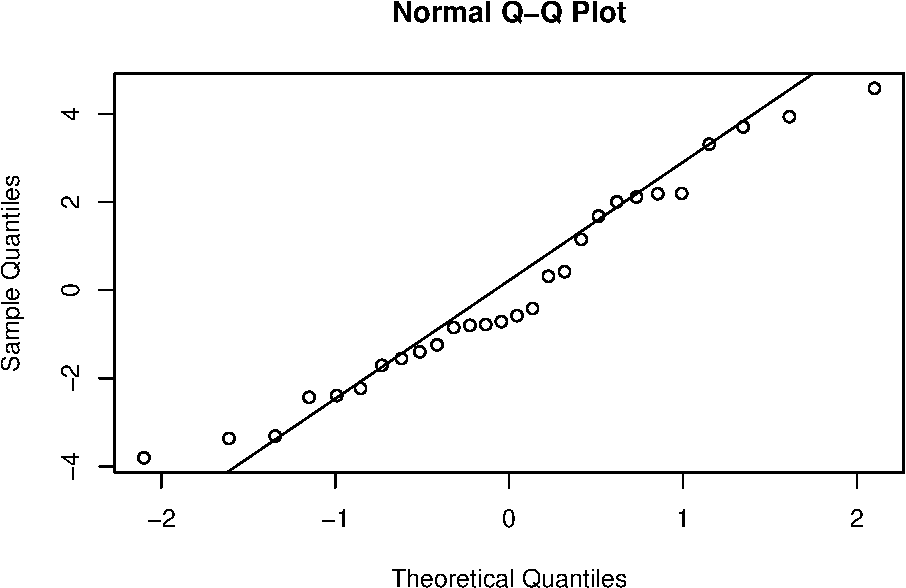
\includegraphics[width=0.9\linewidth]{examples_files/figure-latex/unnamed-chunk-20-1}

It appears that the normality assumption is fine since the standardized
residuals closely follow the theoretical quantiles for a normal
distribution as observered in the quantile-quantile plot.

\subsubsection{Part b.}\label{part-b.-4}

\begin{Shaded}
\begin{Highlighting}[]
\FunctionTok{plot}\NormalTok{(}\FunctionTok{fitted}\NormalTok{(model), residuals, }\AttributeTok{main =} \StringTok{"Residuals vs Fitted Value"}\NormalTok{)}
\FunctionTok{abline}\NormalTok{(}\AttributeTok{h=}\DecValTok{0}\NormalTok{, }\AttributeTok{col =} \StringTok{\textquotesingle{}red\textquotesingle{}}\NormalTok{)}
\end{Highlighting}
\end{Shaded}

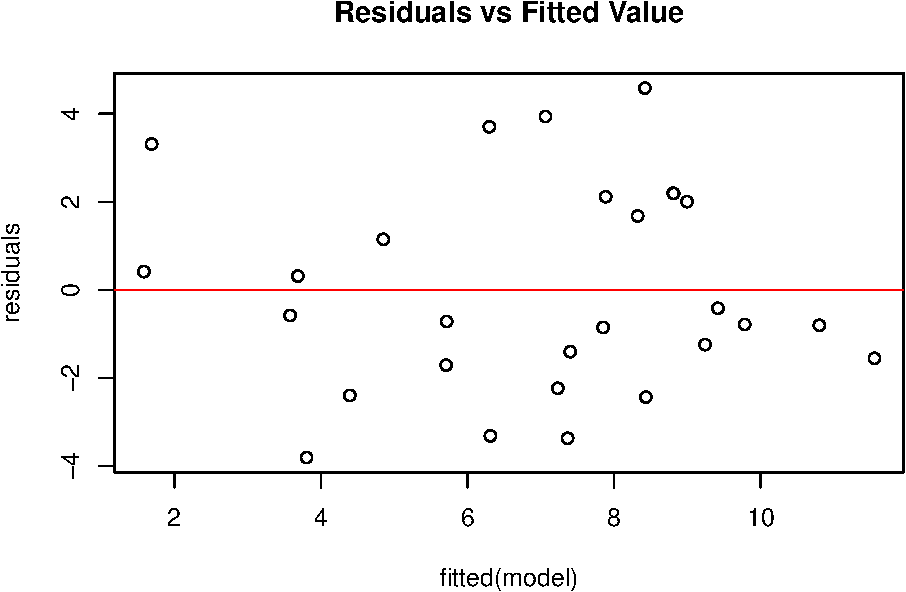
\includegraphics[width=0.75\linewidth]{examples_files/figure-latex/unnamed-chunk-21-1}

The model appears to be adequate since the residuals vs fitted values
appear to be randomly distributed around 0, showing no patterns.

\subsubsection{Part c.}\label{part-c.-3}

\begin{Shaded}
\begin{Highlighting}[]
\NormalTok{residuals }\OtherTok{\textless{}{-}} \FunctionTok{residuals}\NormalTok{(model)}
\FunctionTok{plot}\NormalTok{(tableb1}\SpecialCharTok{$}\NormalTok{x2, residuals, }\AttributeTok{xlab=}\StringTok{"Passing Yardage"}\NormalTok{,}
     \AttributeTok{ylab=}\StringTok{"Residuals"}\NormalTok{, }\AttributeTok{main=}\StringTok{"Residuals vs Team Passing Yardage"}\NormalTok{)}
\FunctionTok{abline}\NormalTok{(}\AttributeTok{h=}\DecValTok{0}\NormalTok{, }\AttributeTok{col=}\StringTok{"red"}\NormalTok{)}
\end{Highlighting}
\end{Shaded}

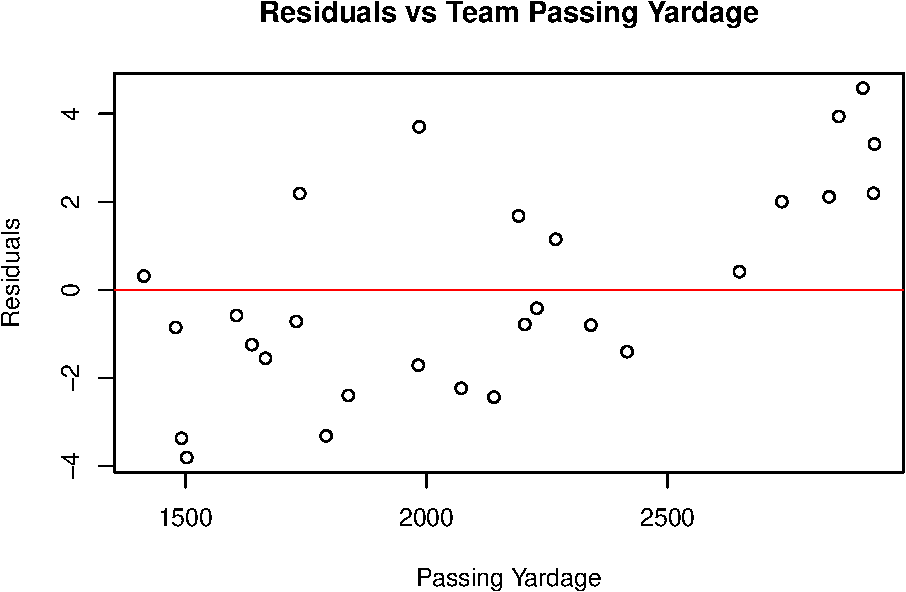
\includegraphics[width=0.75\linewidth]{examples_files/figure-latex/unnamed-chunk-22-1}

The model appears to be improved when adding \(x_2\) since the residuals
appear to be more close to 0.

\subsection{Lack of Fit Example}\label{lack-of-fit-example}

We are going to use this data to conduct a lack of fit test.

\begin{center}
  \begin{tabular}{|c|c|c|c|c|c|c|c|c|c|c|}
    \hline
      x & 1 & 1 & 2 & 3.3 & 3.3 & 4 & 4 & 4 & 4.7 & 5\\
      \hline
      y & 10.84 & 9.30 & 16.35 &22.88  &24.35 & 24.56& 25.86 &29.16 &24.59& 22.25\\
      \hline
      x & 5.6 & 5.6 & 5.6 & 6.0 & 6.0 & 6.5 & 6 & & & \\
      \hline
      y & 25.90 & 27.20 & 25.61 & 25.45 & 26.56 & 21.03 & 21.46 & & & \\
    \hline
  \end{tabular}
\end{center}

We can count that there are \(m= 10\) levels, and \(n=17\) observations,
so \[\sum_{i=1}^n n_i = 2 + 1 + 3 + \cdots = 17\] We can compute then
fit a model with this data in R,

\begin{Shaded}
\begin{Highlighting}[]
\NormalTok{x }\OtherTok{\textless{}{-}} \FunctionTok{c}\NormalTok{(}\DecValTok{1}\NormalTok{,}\DecValTok{1}\NormalTok{,}\DecValTok{2}\NormalTok{,}\FloatTok{3.3}\NormalTok{,}\FloatTok{3.3}\NormalTok{,}\DecValTok{4}\NormalTok{,}\DecValTok{4}\NormalTok{,}\DecValTok{4}\NormalTok{,}\FloatTok{4.7}\NormalTok{,}\DecValTok{5}\NormalTok{,}\FloatTok{5.6}\NormalTok{,}\FloatTok{5.6}\NormalTok{,}\FloatTok{5.6}\NormalTok{,}\DecValTok{6}\NormalTok{,}\DecValTok{6}\NormalTok{,}\FloatTok{6.5}\NormalTok{,}\DecValTok{6}\NormalTok{)}
\NormalTok{y }\OtherTok{\textless{}{-}} \FunctionTok{c}\NormalTok{(}\FloatTok{10.84}\NormalTok{ , }\FloatTok{9.30}\NormalTok{ , }\FloatTok{16.35}\NormalTok{ ,}\FloatTok{22.88}\NormalTok{  ,}\FloatTok{24.35}\NormalTok{ , }\FloatTok{24.56}\NormalTok{, }\FloatTok{25.86}\NormalTok{ ,}\FloatTok{29.16} 
\NormalTok{      ,}\FloatTok{24.59}\NormalTok{, }\FloatTok{22.25}\NormalTok{,}\FloatTok{25.90}\NormalTok{ , }\FloatTok{27.20}\NormalTok{ , }\FloatTok{25.61}\NormalTok{ , }\FloatTok{25.45}\NormalTok{ , }\FloatTok{26.56}\NormalTok{ , }\FloatTok{21.03}\NormalTok{ ,}\FloatTok{21.46}\NormalTok{)}
\NormalTok{model }\OtherTok{\textless{}{-}} \FunctionTok{lm}\NormalTok{(}\AttributeTok{formula =}\NormalTok{ y }\SpecialCharTok{\textasciitilde{}}\NormalTok{ x)}
\FunctionTok{print}\NormalTok{(model)}
\end{Highlighting}
\end{Shaded}

\begin{verbatim}
## 
## Call:
## lm(formula = y ~ x)
## 
## Coefficients:
## (Intercept)            x  
##      12.523        2.316
\end{verbatim}

\begin{Shaded}
\begin{Highlighting}[]
\FunctionTok{anova}\NormalTok{(model)}
\end{Highlighting}
\end{Shaded}

\begin{verbatim}
## Analysis of Variance Table
## 
## Response: y
##           Df Sum Sq Mean Sq F value    Pr(>F)    
## x          1 260.44 260.439  17.196 0.0008606 ***
## Residuals 15 227.17  15.145                      
## ---
## Signif. codes:  0 '***' 0.001 '**' 0.01 '*' 0.05 '.' 0.1 ' ' 1
\end{verbatim}

We get the linear model \[\hat{y}_i = 12.5323 + 2.316x_i\]

Then, we can compute lack of fit and pure error with
\[SS_{PE} = \sum_{i=1}^m\sum_{j=1}^{n_i} (y_{ij} - \bar{y}_i)^2, SS_{LOF} = SSE - SS_{PE}\]
In R, we get

\begin{Shaded}
\begin{Highlighting}[]
\FunctionTok{library}\NormalTok{(EnvStats)}
\FunctionTok{anovaPE}\NormalTok{(model)}
\end{Highlighting}
\end{Shaded}

\begin{verbatim}
##              Df  Sum Sq Mean Sq F value    Pr(>F)    
## x             1 260.439 260.439 71.0262 2.996e-05 ***
## Lack of Fit   7 197.840  28.263  7.7078  0.004971 ** 
## Pure Error    8  29.334   3.667                      
## ---
## Signif. codes:  0 '***' 0.001 '**' 0.01 '*' 0.05 '.' 0.1 ' ' 1
\end{verbatim}

Our \(F\)-statistic is 7.70, and the critical value is
\(F_{\alpha, m-2, n-m}\), which we can compute in R or look at a table.

\begin{Shaded}
\begin{Highlighting}[]
\FunctionTok{qf}\NormalTok{(}\FloatTok{0.05}\NormalTok{, }\DecValTok{8}\NormalTok{, }\DecValTok{7}\NormalTok{, }\AttributeTok{lower.tail=}\ConstantTok{FALSE}\NormalTok{)}
\end{Highlighting}
\end{Shaded}

\begin{verbatim}
## [1] 3.725725
\end{verbatim}

Therefore, we reject the null hypothesis
\(H_0: E(y_i) = \beta_0 + \beta_1x_i\).

\section{Interprolating Values From Look-up
Table}\label{interprolating-values-from-look-up-table}

Say we want to find the \(t\)-value for \(t_{\alpha_0}\) where
\(\alpha_0\) is not located on the look up table, we then choose the 2
closest \(\alpha\) values, call them \(\alpha_1, \alpha_2\), so that
\(\alpha_1 < \alpha_0 < \alpha_2\). Then, we use the following formula
to interprolate the \(t\)-value as
\[t_{\alpha_0} \approx t_{\alpha_1} + \frac{(\alpha_0 - \alpha_1)(t_{\alpha_2} - t_{\alpha_1})}{\alpha_2 - \alpha_1}\]

\subsection{Example.}\label{example.}

Suppose you have the critical value \(\alpha_0 = 0.015\), the 2 closest
values would be \(\alpha_1 = 0.01\), and \(\alpha_2 = 0.025\). So, we
get
\[t_{0.015} \approx \frac{(0.015 - 0.01)(t_{0.025} - t_{0.01})}{0.025 - 0.01}\]

\begin{Shaded}
\begin{Highlighting}[]
\NormalTok{noint }\OtherTok{\textless{}{-}} \FunctionTok{lm}\NormalTok{(}\AttributeTok{formula =}\NormalTok{ y}\SpecialCharTok{\textasciitilde{}} \DecValTok{0}\NormalTok{)}
\FunctionTok{print}\NormalTok{(noint)}
\end{Highlighting}
\end{Shaded}

\begin{verbatim}
## 
## Call:
## lm(formula = y ~ 0)
## 
## No coefficients
\end{verbatim}

\begin{Shaded}
\begin{Highlighting}[]
\FunctionTok{anova}\NormalTok{(noint)}
\end{Highlighting}
\end{Shaded}

\begin{verbatim}
## Analysis of Variance Table
## 
## Response: y
##           Df Sum Sq Mean Sq F value Pr(>F)
## Residuals 17 9132.2  537.19
\end{verbatim}

\section{Chapter 5 - Weighted Least Squared and
Transformations}\label{chapter-5---weighted-least-squared-and-transformations}

\subsection{Example of checking for model adequecy with BP
test}\label{example-of-checking-for-model-adequecy-with-bp-test}

Using the delivery time data, we can examine the model adequecy of

\begin{Shaded}
\begin{Highlighting}[]
\NormalTok{delivery }\OtherTok{\textless{}{-}} \FunctionTok{read.table}\NormalTok{(}\StringTok{"./Data/delivery.txt"}\NormalTok{,}\AttributeTok{header=}\ConstantTok{TRUE}\NormalTok{, }\AttributeTok{sep=}\StringTok{\textquotesingle{}}\SpecialCharTok{\textbackslash{}t}\StringTok{\textquotesingle{}}\NormalTok{)}
\NormalTok{X1 }\OtherTok{=}\NormalTok{ delivery}\SpecialCharTok{$}\NormalTok{Number.of.Cases}
\NormalTok{X2 }\OtherTok{=}\NormalTok{ delivery}\SpecialCharTok{$}\NormalTok{Distance}
\NormalTok{Y }\OtherTok{=}\NormalTok{ delivery}\SpecialCharTok{$}\NormalTok{Delivery.Time}
\NormalTok{fit }\OtherTok{=} \FunctionTok{lm}\NormalTok{(Y}\SpecialCharTok{\textasciitilde{}}\NormalTok{X1}\SpecialCharTok{+}\NormalTok{X2, }\AttributeTok{data=}\NormalTok{delivery)}
\FunctionTok{par}\NormalTok{(}\AttributeTok{mfrow=}\FunctionTok{c}\NormalTok{(}\DecValTok{2}\NormalTok{,}\DecValTok{2}\NormalTok{))}
\FunctionTok{plot}\NormalTok{(fit)}
\end{Highlighting}
\end{Shaded}

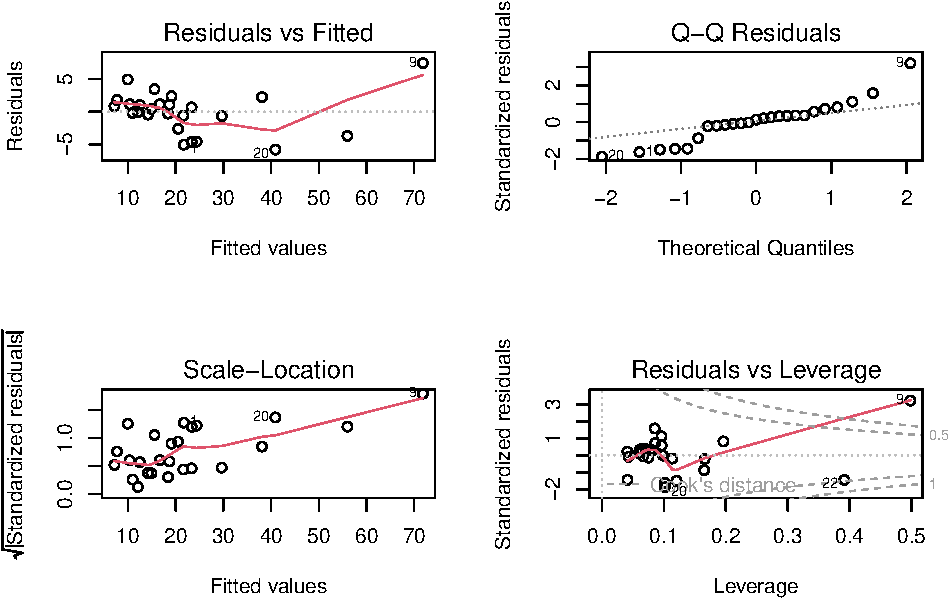
\includegraphics{examples_files/figure-latex/unnamed-chunk-27-1.pdf}

We can see in the qq-plot that the residuals do not follow the
theoretical quantiles of a normal distribution, so there is likely an
issue with the normality assumption of the model. The residuals vs
fitted appear to have some pattern resembling a parabola.

\begin{Shaded}
\begin{Highlighting}[]
\FunctionTok{library}\NormalTok{(lmtest)}
\FunctionTok{bptest}\NormalTok{(fit)}
\end{Highlighting}
\end{Shaded}

\begin{verbatim}
## 
##  studentized Breusch-Pagan test
## 
## data:  fit
## BP = 11.988, df = 2, p-value = 0.002493
\end{verbatim}

We can see that the p-value that it is low, so we reject the null
hypothesis that the variance is constant. We can attempt to remede the
issue with the residuals by applying a boxcox transformation.

\begin{Shaded}
\begin{Highlighting}[]
\FunctionTok{library}\NormalTok{(MASS)}
\FunctionTok{boxcox}\NormalTok{(fit)}
\NormalTok{b }\OtherTok{\textless{}{-}} \FunctionTok{boxcox}\NormalTok{(fit)}
\end{Highlighting}
\end{Shaded}

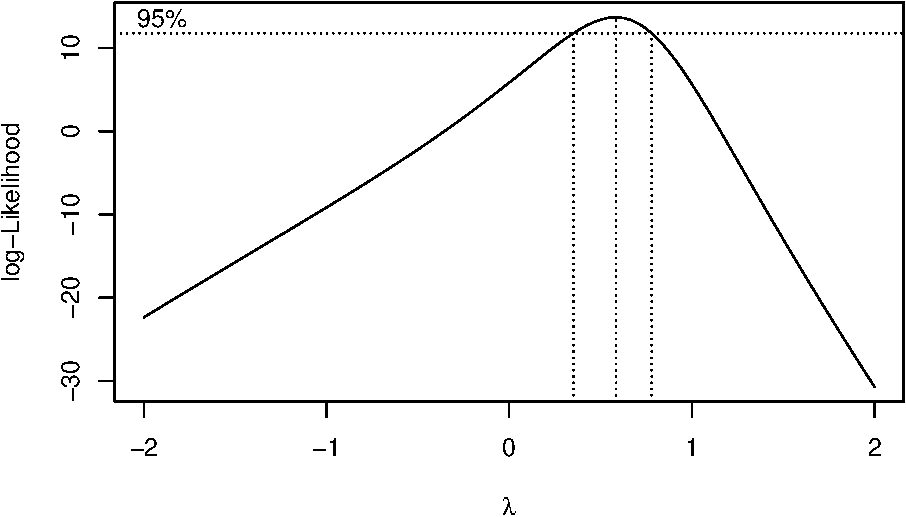
\includegraphics{examples_files/figure-latex/unnamed-chunk-29-1.pdf}

\begin{Shaded}
\begin{Highlighting}[]
\NormalTok{lambda }\OtherTok{\textless{}{-}}\NormalTok{ b}\SpecialCharTok{$}\NormalTok{x[}\FunctionTok{which.max}\NormalTok{(}\FunctionTok{boxcox}\NormalTok{(fit)}\SpecialCharTok{$}\NormalTok{y)]}
\NormalTok{lambda}
\end{Highlighting}
\end{Shaded}

\begin{verbatim}
## [1] 0.5858586
\end{verbatim}

Now using our lambda value, we can transform \(y\) and refit the model,

\begin{Shaded}
\begin{Highlighting}[]
\NormalTok{n }\OtherTok{=} \FunctionTok{length}\NormalTok{(Y)}

\NormalTok{y\_dot }\OtherTok{\textless{}{-}} \FunctionTok{exp}\NormalTok{(}\DecValTok{1}\SpecialCharTok{/}\NormalTok{n }\SpecialCharTok{*} \FunctionTok{sum}\NormalTok{(}\FunctionTok{log}\NormalTok{(Y)))}

\NormalTok{Y\_transformed }\OtherTok{\textless{}{-}}\NormalTok{ (Y}\SpecialCharTok{\^{}}\NormalTok{lambda }\SpecialCharTok{{-}} \DecValTok{1}\NormalTok{) }\SpecialCharTok{/}\NormalTok{ (lambda }\SpecialCharTok{*}\NormalTok{ y\_dot}\SpecialCharTok{\^{}}\NormalTok{(lambda }\SpecialCharTok{{-}} \DecValTok{1}\NormalTok{))}

\NormalTok{new\_model }\OtherTok{\textless{}{-}} \FunctionTok{lm}\NormalTok{(Y\_transformed }\SpecialCharTok{\textasciitilde{}}\NormalTok{ X1 }\SpecialCharTok{+}\NormalTok{ X2, }\AttributeTok{data=}\NormalTok{delivery)}

\FunctionTok{par}\NormalTok{(}\AttributeTok{mfrow=}\FunctionTok{c}\NormalTok{(}\DecValTok{2}\NormalTok{,}\DecValTok{2}\NormalTok{))}

\FunctionTok{plot}\NormalTok{(new\_model)}
\end{Highlighting}
\end{Shaded}

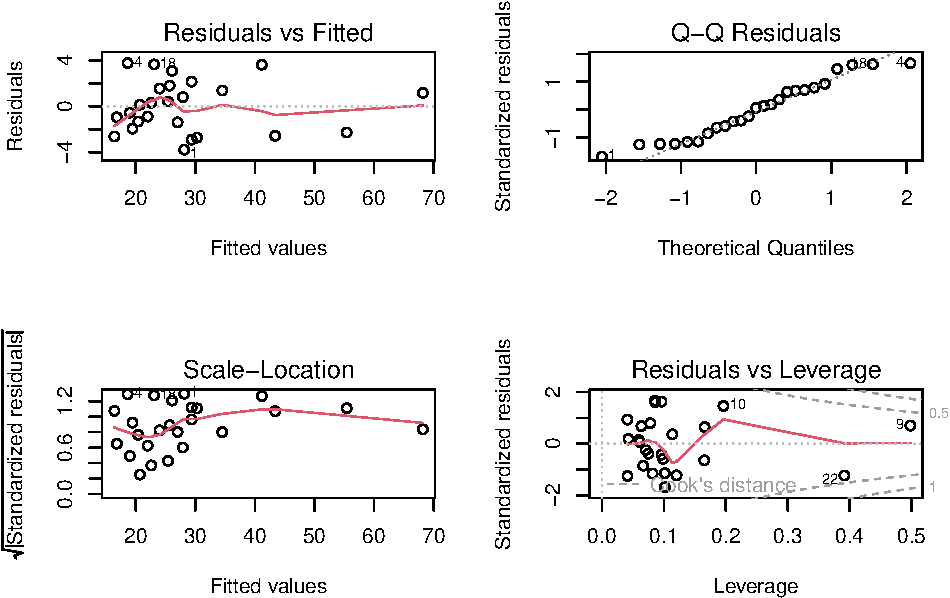
\includegraphics{examples_files/figure-latex/unnamed-chunk-30-1.pdf}

We can see that the qq-plot looks better now and the residuals appear
fairly normally distributed, as well as the residuals vs fitted look
more random, so we also can conclude that there is no longer an issue
with the constant variance assumption. Another approach to this problem
is to use another transformation on \(y\). Since the reponse variable
\(y\) is the time, which is count, the simplest probabilistic model for
count data is the Poisson distribution, thus we transform
\(y' = \sqrt{y}\), and we plot this model.

\begin{Shaded}
\begin{Highlighting}[]
\NormalTok{y\_prime }\OtherTok{\textless{}{-}} \FunctionTok{sqrt}\NormalTok{(Y)}

\NormalTok{sqrt\_y\_model }\OtherTok{\textless{}{-}} \FunctionTok{lm}\NormalTok{(y\_prime }\SpecialCharTok{\textasciitilde{}}\NormalTok{ X1 }\SpecialCharTok{+}\NormalTok{ X2, }\AttributeTok{data=}\NormalTok{delivery)}

\FunctionTok{par}\NormalTok{(}\AttributeTok{mfrow=}\FunctionTok{c}\NormalTok{(}\DecValTok{2}\NormalTok{,}\DecValTok{2}\NormalTok{))}

\FunctionTok{plot}\NormalTok{(sqrt\_y\_model)}
\end{Highlighting}
\end{Shaded}

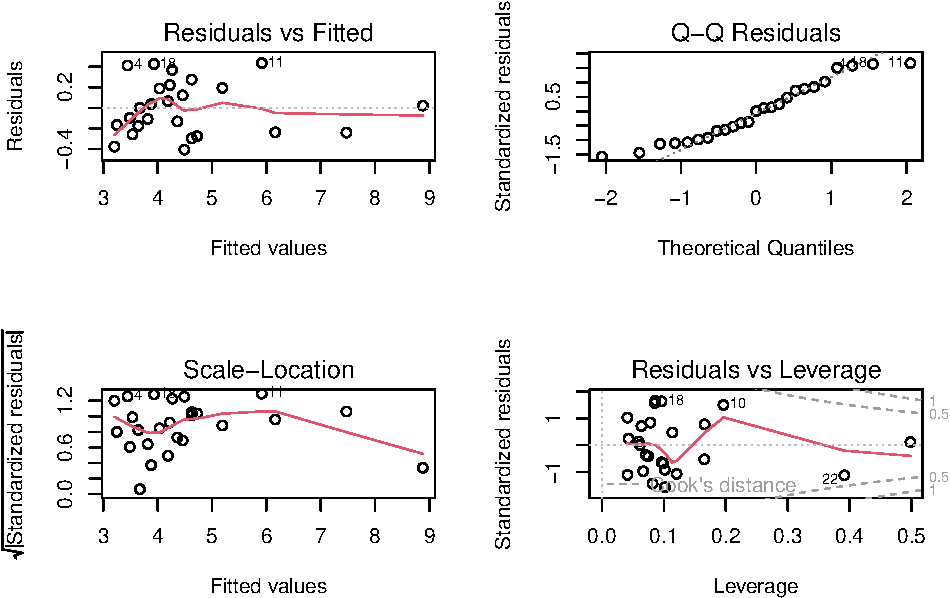
\includegraphics{examples_files/figure-latex/unnamed-chunk-31-1.pdf}

We see that we get fairly similar results to the boxcox transformation,
and can conlude the assumption of constant variance is no longer
violated.

\subsection{Example of Weighted Least
Squares}\label{example-of-weighted-least-squares}

Using the weighted Turkey data, we can fit a model an examine the
residuals.

\begin{Shaded}
\begin{Highlighting}[]
\NormalTok{turkey }\OtherTok{\textless{}{-}} \FunctionTok{read.table}\NormalTok{(}\StringTok{"./Data/weighted.txt"}\NormalTok{,}\AttributeTok{header=}\ConstantTok{TRUE}\NormalTok{, }\AttributeTok{sep=}\StringTok{\textquotesingle{}}\SpecialCharTok{\textbackslash{}t}\StringTok{\textquotesingle{}}\NormalTok{)}



\NormalTok{fit }\OtherTok{\textless{}{-}} \FunctionTok{lm}\NormalTok{(Y }\SpecialCharTok{\textasciitilde{}}\NormalTok{ X, }\AttributeTok{data=}\NormalTok{turkey)}

\FunctionTok{summary}\NormalTok{(fit)}
\end{Highlighting}
\end{Shaded}

\begin{verbatim}
## 
## Call:
## lm(formula = Y ~ X, data = turkey)
## 
## Residuals:
##     Min      1Q  Median      3Q     Max 
## -4.0928 -0.6087 -0.0473  1.1256  2.4238 
## 
## Coefficients:
##             Estimate Std. Error t value Pr(>|t|)    
## (Intercept) -0.57895    0.67919  -0.852      0.4    
## X            1.13540    0.08622  13.169 1.09e-14 ***
## ---
## Signif. codes:  0 '***' 0.001 '**' 0.01 '*' 0.05 '.' 0.1 ' ' 1
## 
## Residual standard error: 1.457 on 33 degrees of freedom
## Multiple R-squared:  0.8401, Adjusted R-squared:  0.8353 
## F-statistic: 173.4 on 1 and 33 DF,  p-value: 1.089e-14
\end{verbatim}

\begin{Shaded}
\begin{Highlighting}[]
\FunctionTok{plot}\NormalTok{(fit,}\DecValTok{1}\NormalTok{)}
\end{Highlighting}
\end{Shaded}

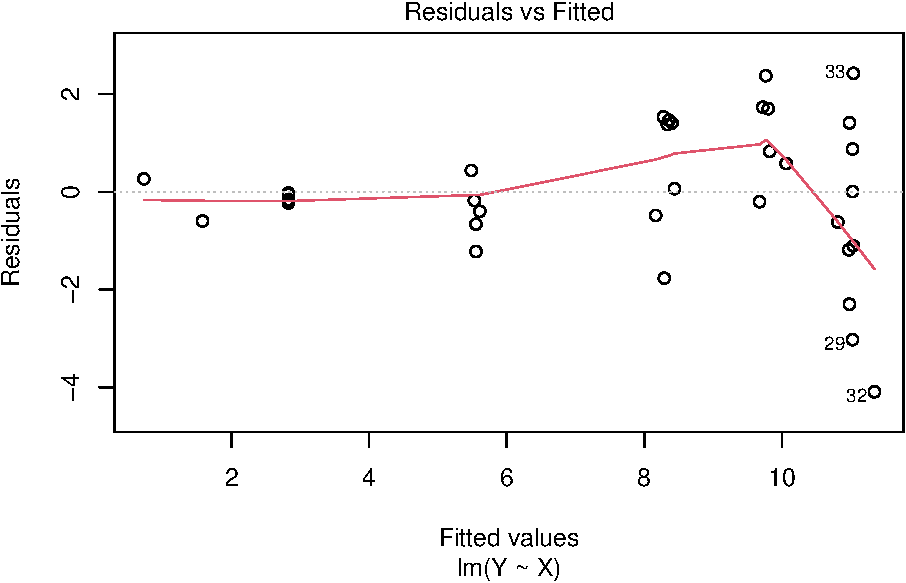
\includegraphics{examples_files/figure-latex/unnamed-chunk-32-1.pdf}

As we can see, there appears to be a telescoping effect. One way to
proceed is to perform the usual regression. Then, group the data using
the X variable. Estimate the variances \(s^2_i\) of the \(Y_i\) for each
group. Then fit the variances against the averages of the \(X_i\) of the
groups. Next we computed averages and variances for subsets of the data
and then fitted the variances against the averages.

\begin{Shaded}
\begin{Highlighting}[]
\NormalTok{turkey}
\end{Highlighting}
\end{Shaded}

\begin{verbatim}
##        X     Y
## 1   1.15  0.99
## 2   1.90  0.98
## 3   3.00  2.60
## 4   3.00  2.67
## 5   3.00  2.66
## 6   3.00  2.78
## 7   3.00  2.80
## 8   5.34  5.92
## 9   5.38  5.35
## 10  5.40  4.33
## 11  5.40  4.89
## 12  5.45  5.21
## 13  7.70  7.68
## 14  7.80  9.81
## 15  7.81  6.52
## 16  7.85  9.71
## 17  7.87  9.82
## 18  7.91  9.81
## 19  7.94  8.50
## 20  9.03  9.47
## 21  9.07 11.45
## 22  9.11 12.14
## 23  9.14 11.50
## 24  9.16 10.65
## 25  9.37 10.64
## 26 10.17  9.78
## 27 10.18 12.39
## 28 10.22 11.03
## 29 10.22  8.00
## 30 10.22 11.90
## 31 10.18  8.68
## 32 10.50  7.25
## 33 10.23 13.46
## 34 10.03 10.19
## 35 10.23  9.93
\end{verbatim}

We can see that we have many data points at 3, 5.4, 7.8, 9.1, and 10.2.
These aren't perfect groupings but there are many points at this \(X\)
value or very close to it, so we will use these as our groups. Now we
can compute the variances at each of these points.

\begin{Shaded}
\begin{Highlighting}[]
\NormalTok{s1 }\OtherTok{\textless{}{-}} \FunctionTok{round}\NormalTok{(}\FunctionTok{var}\NormalTok{(turkey[turkey}\SpecialCharTok{$}\NormalTok{X }\SpecialCharTok{==} \DecValTok{3}\NormalTok{, ]}\SpecialCharTok{$}\NormalTok{Y),}\DecValTok{4}\NormalTok{)}
\NormalTok{s2 }\OtherTok{\textless{}{-}} \FunctionTok{round}\NormalTok{(}\FunctionTok{var}\NormalTok{(}\FunctionTok{subset}\NormalTok{(turkey, X }\SpecialCharTok{\textgreater{}=} \FloatTok{5.34} \SpecialCharTok{\&}\NormalTok{ X }\SpecialCharTok{\textless{}=} \FloatTok{5.45}\NormalTok{)}\SpecialCharTok{$}\NormalTok{Y),}\DecValTok{4}\NormalTok{)}
\NormalTok{s3 }\OtherTok{\textless{}{-}} \FunctionTok{round}\NormalTok{(}\FunctionTok{var}\NormalTok{(}\FunctionTok{subset}\NormalTok{(turkey, X }\SpecialCharTok{\textgreater{}=} \FloatTok{7.7} \SpecialCharTok{\&}\NormalTok{ X }\SpecialCharTok{\textless{}=} \FloatTok{7.94}\NormalTok{)}\SpecialCharTok{$}\NormalTok{Y),}\DecValTok{4}\NormalTok{)}
\NormalTok{s4 }\OtherTok{\textless{}{-}} \FunctionTok{round}\NormalTok{(}\FunctionTok{var}\NormalTok{(}\FunctionTok{subset}\NormalTok{(turkey, X }\SpecialCharTok{\textgreater{}=} \FloatTok{9.03} \SpecialCharTok{\&}\NormalTok{ X }\SpecialCharTok{\textless{}=} \FloatTok{9.37}\NormalTok{)}\SpecialCharTok{$}\NormalTok{Y),}\DecValTok{4}\NormalTok{)}
\NormalTok{s5 }\OtherTok{\textless{}{-}} \FunctionTok{round}\NormalTok{(}\FunctionTok{var}\NormalTok{(}\FunctionTok{subset}\NormalTok{(turkey, X }\SpecialCharTok{\textgreater{}=} \FloatTok{10.03} \SpecialCharTok{\&}\NormalTok{ X }\SpecialCharTok{\textless{}=} \FloatTok{10.5}\NormalTok{)}\SpecialCharTok{$}\NormalTok{Y),}\DecValTok{4}\NormalTok{)}

\NormalTok{s }\OtherTok{\textless{}{-}} \FunctionTok{c}\NormalTok{(s1, s2, s3, s4, s5)}

\NormalTok{df }\OtherTok{\textless{}{-}} \FunctionTok{data.frame}\NormalTok{(}\AttributeTok{X =} \FunctionTok{c}\NormalTok{(}\DecValTok{3}\NormalTok{, }\FloatTok{5.4}\NormalTok{, }\FloatTok{7.8}\NormalTok{, }\FloatTok{9.1}\NormalTok{, }\FloatTok{10.2}\NormalTok{), }\AttributeTok{s =}\NormalTok{ s)}
\NormalTok{df}
\end{Highlighting}
\end{Shaded}

\begin{verbatim}
##      X      s
## 1  3.0 0.0072
## 2  5.4 0.3440
## 3  7.8 1.7404
## 4  9.1 0.8683
## 5 10.2 3.8964
\end{verbatim}

So now that we have our dataframe, we can fit a model with \(s\) as the
response and the averages that we picked,

\begin{Shaded}
\begin{Highlighting}[]
\NormalTok{fit2 }\OtherTok{\textless{}{-}} \FunctionTok{lm}\NormalTok{(s }\SpecialCharTok{\textasciitilde{}}\NormalTok{ X }\SpecialCharTok{+} \FunctionTok{I}\NormalTok{(X}\SpecialCharTok{\^{}}\DecValTok{2}\NormalTok{), }\AttributeTok{data=}\NormalTok{df)}
\FunctionTok{summary}\NormalTok{(fit2)}
\end{Highlighting}
\end{Shaded}

\begin{verbatim}
## 
## Call:
## lm(formula = s ~ X + I(X^2), data = df)
## 
## Residuals:
##       1       2       3       4       5 
## -0.1198  0.1980  0.5586 -1.2990  0.6621 
## 
## Coefficients:
##             Estimate Std. Error t value Pr(>|t|)
## (Intercept)  1.53291    3.78395   0.405    0.725
## X           -0.73343    1.28494  -0.571    0.626
## I(X^2)       0.08826    0.09666   0.913    0.458
## 
## Residual standard error: 1.116 on 2 degrees of freedom
## Multiple R-squared:  0.7427, Adjusted R-squared:  0.4853 
## F-statistic: 2.886 on 2 and 2 DF,  p-value: 0.2573
\end{verbatim}

Now, we have the regression model

\[\hat{s}^2 = 1.5329 - 0.7334\bar{X} + 0.0883\bar{X}^2\]

The weights are then computes as inverses of the predicted variances,

\begin{Shaded}
\begin{Highlighting}[]
\NormalTok{weights }\OtherTok{\textless{}{-}} \DecValTok{1}\SpecialCharTok{/}\FunctionTok{predict}\NormalTok{(fit2, }\AttributeTok{newdata =} \FunctionTok{data.frame}\NormalTok{(}\AttributeTok{X =}\NormalTok{ turkey}\SpecialCharTok{$}\NormalTok{X))}

\NormalTok{weighted\_model }\OtherTok{\textless{}{-}} \FunctionTok{lm}\NormalTok{(Y }\SpecialCharTok{\textasciitilde{}}\NormalTok{ X, }\AttributeTok{data=}\NormalTok{turkey, }\AttributeTok{weights=}\NormalTok{weights)}
\FunctionTok{summary}\NormalTok{(weighted\_model)}
\end{Highlighting}
\end{Shaded}

\begin{verbatim}
## 
## Call:
## lm(formula = Y ~ X, data = turkey, weights = weights)
## 
## Weighted Residuals:
##     Min      1Q  Median      3Q     Max 
## -2.8010 -0.5572  0.1544  0.9843  1.6397 
## 
## Coefficients:
##             Estimate Std. Error t value Pr(>|t|)    
## (Intercept) -0.88908    0.30058  -2.958  0.00569 ** 
## X            1.16469    0.05945  19.590  < 2e-16 ***
## ---
## Signif. codes:  0 '***' 0.001 '**' 0.01 '*' 0.05 '.' 0.1 ' ' 1
## 
## Residual standard error: 1.139 on 33 degrees of freedom
## Multiple R-squared:  0.9208, Adjusted R-squared:  0.9184 
## F-statistic: 383.8 on 1 and 33 DF,  p-value: < 2.2e-16
\end{verbatim}

The original model was

\[\hat{Y} = -0.579 + 1.14 X\]

The new weighted model becomes

\[\hat{Y} = -0.89 + 1.16 X\]

\section{Chapter 6 - Regression Diagnostics and Measures of
Influence}\label{chapter-6---regression-diagnostics-and-measures-of-influence}

We will examine the bank dataset and fit a model to the data. Then
examine the residuals and look for any outliers or influential points.

\begin{Shaded}
\begin{Highlighting}[]
\FunctionTok{library}\NormalTok{(olsrr)}
\end{Highlighting}
\end{Shaded}

\begin{verbatim}
## 
## Attaching package: 'olsrr'
\end{verbatim}

\begin{verbatim}
## The following object is masked from 'package:MASS':
## 
##     cement
\end{verbatim}

\begin{verbatim}
## The following object is masked from 'package:MPV':
## 
##     cement
\end{verbatim}

\begin{verbatim}
## The following object is masked from 'package:datasets':
## 
##     rivers
\end{verbatim}

\begin{Shaded}
\begin{Highlighting}[]
\NormalTok{bank }\OtherTok{\textless{}{-}} \FunctionTok{read.table}\NormalTok{(}\StringTok{"./Data/bank.txt"}\NormalTok{,}\AttributeTok{header=}\ConstantTok{TRUE}\NormalTok{, }\AttributeTok{sep=}\StringTok{\textquotesingle{}}\SpecialCharTok{\textbackslash{}t}\StringTok{\textquotesingle{}}\NormalTok{)}

\NormalTok{y }\OtherTok{\textless{}{-}}\NormalTok{ bank}\SpecialCharTok{$}\NormalTok{Number.New.accounts}
\NormalTok{x }\OtherTok{\textless{}{-}}\NormalTok{ bank}\SpecialCharTok{$}\NormalTok{Minimum.Deposit}
\NormalTok{fit }\OtherTok{\textless{}{-}} \FunctionTok{lm}\NormalTok{(y}\SpecialCharTok{\textasciitilde{}}\NormalTok{x)}
\CommentTok{\# Cook\textquotesingle{}s Distance vs. Observations}
\FunctionTok{ols\_plot\_cooksd\_bar}\NormalTok{(fit)}
\end{Highlighting}
\end{Shaded}

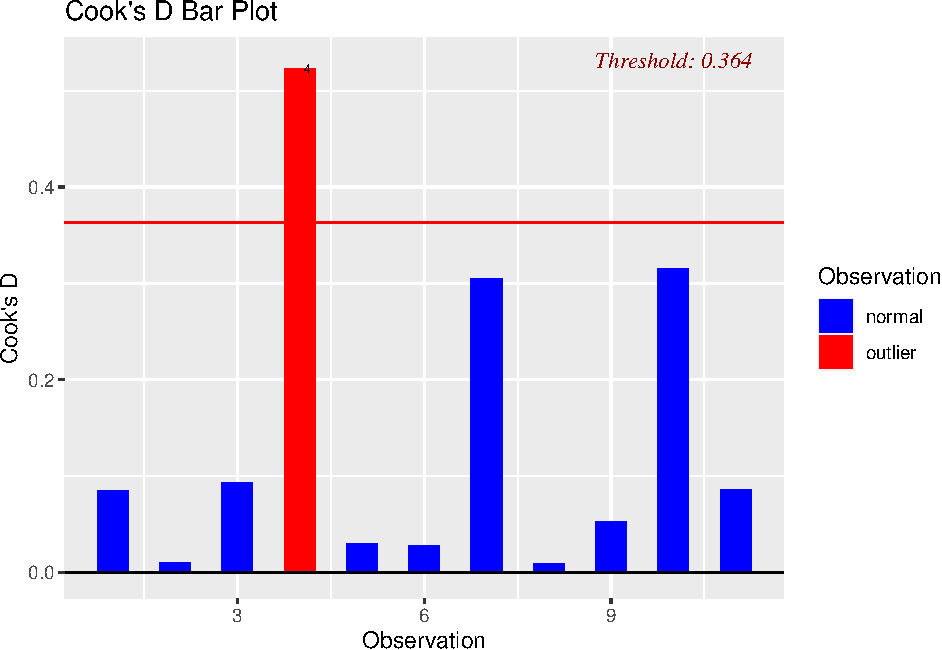
\includegraphics{examples_files/figure-latex/unnamed-chunk-37-1.pdf}

From the Cook's distant plot, we see that the 4th observation is
influential on the fitted values at all \(X\) values. We can look at the
plot for DFFITS,

\begin{Shaded}
\begin{Highlighting}[]
\FunctionTok{ols\_plot\_dffits}\NormalTok{(fit)}
\end{Highlighting}
\end{Shaded}

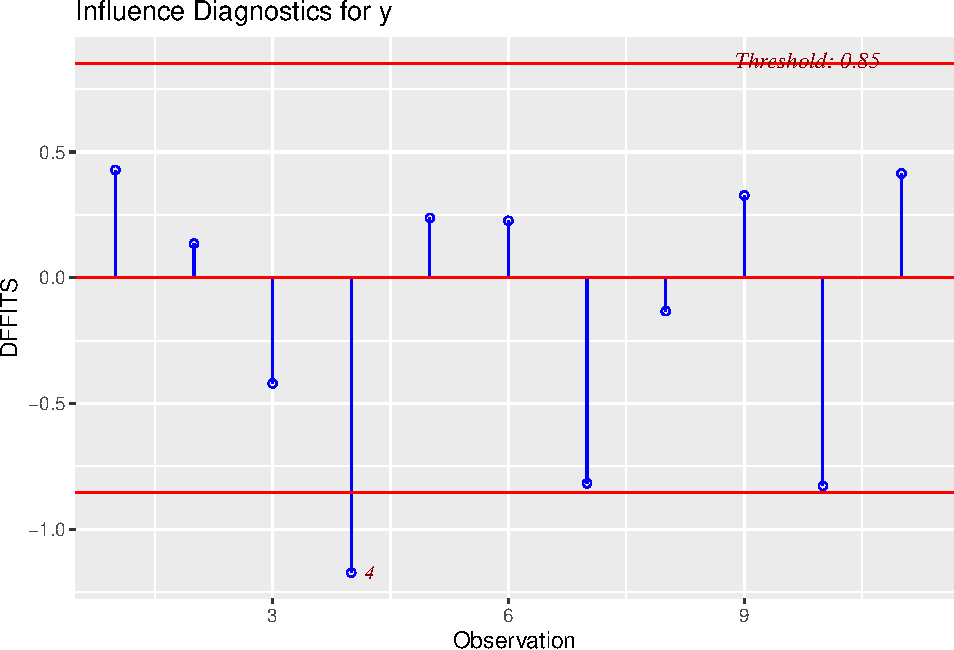
\includegraphics{examples_files/figure-latex/unnamed-chunk-38-1.pdf}

We see again that the 4th observation is influential on the 4th fitted
value of the model. We can also look at the DFBETAS plot,

\begin{Shaded}
\begin{Highlighting}[]
\FunctionTok{ols\_plot\_dfbetas}\NormalTok{(fit)}
\end{Highlighting}
\end{Shaded}

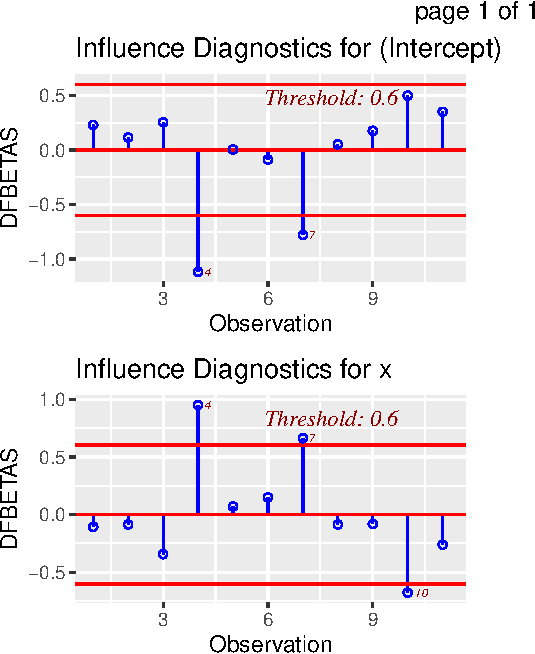
\includegraphics{examples_files/figure-latex/unnamed-chunk-39-1.pdf}

From the DFBETAS vs Observation plots, we see that the 4th, 7th, and
10th observations are influential on the slope, and the 4th and 7th
oberservations are influential on the intercept. To summarize, we can
examine the measures of influence with

\begin{Shaded}
\begin{Highlighting}[]
\FunctionTok{influence.measures}\NormalTok{(fit)}
\end{Highlighting}
\end{Shaded}

\begin{verbatim}
## Influence measures of
##   lm(formula = y ~ x) :
## 
##      dfb.1_   dfb.x  dffit cov.r  cook.d    hat inf
## 1   0.22952 -0.1062  0.428 0.951 0.08506 0.0969    
## 2   0.11433 -0.0860  0.136 1.454 0.01024 0.1518    
## 3   0.25317 -0.3446 -0.420 1.566 0.09395 0.2775    
## 4  -1.11603  0.9498 -1.173 0.787 0.52318 0.2644   *
## 5   0.00406  0.0698  0.238 1.241 0.02993 0.0995    
## 6  -0.08838  0.1486  0.226 1.409 0.02790 0.1597    
## 7  -0.77818  0.6623 -0.818 1.133 0.30507 0.2644    
## 8   0.05173 -0.0870 -0.133 1.472 0.00977 0.1597    
## 9   0.17533 -0.0811  0.327 1.108 0.05356 0.0969    
## 10  0.49853 -0.6786 -0.828 1.171 0.31504 0.2775    
## 11  0.34910 -0.2626  0.415 1.189 0.08634 0.1518
\end{verbatim}

\section{Chapter 7 - Polynomial and Indicator
Regression}\label{chapter-7---polynomial-and-indicator-regression}

\subsection{Example using Indicator
Variables}\label{example-using-indicator-variables}

We will use the turkey dataset

\begin{Shaded}
\begin{Highlighting}[]
\NormalTok{turkey }\OtherTok{\textless{}{-}} \FunctionTok{read.table}\NormalTok{(}\StringTok{"./Data/turkey.txt"}\NormalTok{,}\AttributeTok{header=}\ConstantTok{TRUE}\NormalTok{, }\AttributeTok{sep=}\StringTok{\textquotesingle{}}\SpecialCharTok{\textbackslash{}t}\StringTok{\textquotesingle{}}\NormalTok{)}
\NormalTok{turkey}
\end{Highlighting}
\end{Shaded}

\begin{verbatim}
##    Age Weight Origin Z1 Z2
## 1   28   13.3      G  1  0
## 2   20    8.9      G  1  0
## 3   32   15.1      G  1  0
## 4   22   10.4      G  1  0
## 5   29   13.1      V  0  1
## 6   27   12.4      V  0  1
## 7   28   13.2      V  0  1
## 8   26   11.8      V  0  1
## 9   21   11.5      W  0  0
## 10  27   14.2      W  0  0
## 11  29   15.4      W  0  0
## 12  23   13.1      W  0  0
## 13  25   13.8      W  0  0
\end{verbatim}

We can see that we have a catagorical variable ``origin'', which has 3
levels, G, V, and W. So, we create 2 dummy variables \(Z_1\) and \(Z_2\)
to represent the levels. In this case, it was done for us with
\((Z_1, Z_2) = (0,0) \implies W\), \((Z_1, Z_2) = (0,1) \implies V\),
and \((Z_1, Z_2) = (1,0) \implies G\). 1 dummy variables allows for
\(2^1 = 2\) levels, 2 dummy variables gives us \(2^{2} = 4\) levels, and
so on.

We can plot a model using just age and weight,

\begin{Shaded}
\begin{Highlighting}[]
\NormalTok{model1 }\OtherTok{\textless{}{-}} \FunctionTok{lm}\NormalTok{(Weight }\SpecialCharTok{\textasciitilde{}}\NormalTok{ Age, }\AttributeTok{data=}\NormalTok{turkey)}
\FunctionTok{summary}\NormalTok{(model1) }
\end{Highlighting}
\end{Shaded}

\begin{verbatim}
## 
## Call:
## lm(formula = Weight ~ Age, data = turkey)
## 
## Residuals:
##     Min      1Q  Median      3Q     Max 
## -1.4167 -0.8333 -0.3500  0.9667  1.5333 
## 
## Coefficients:
##             Estimate Std. Error t value Pr(>|t|)    
## (Intercept)  1.98333    2.33273    0.85 0.413327    
## Age          0.41667    0.08922    4.67 0.000682 ***
## ---
## Signif. codes:  0 '***' 0.001 '**' 0.01 '*' 0.05 '.' 0.1 ' ' 1
## 
## Residual standard error: 1.096 on 11 degrees of freedom
## Multiple R-squared:  0.6647, Adjusted R-squared:  0.6343 
## F-statistic: 21.81 on 1 and 11 DF,  p-value: 0.0006824
\end{verbatim}

We see that there is a significant relationship between age and weight,
the \(R^2\) value is a bit low at 0.66, we can examine the model
adequency.

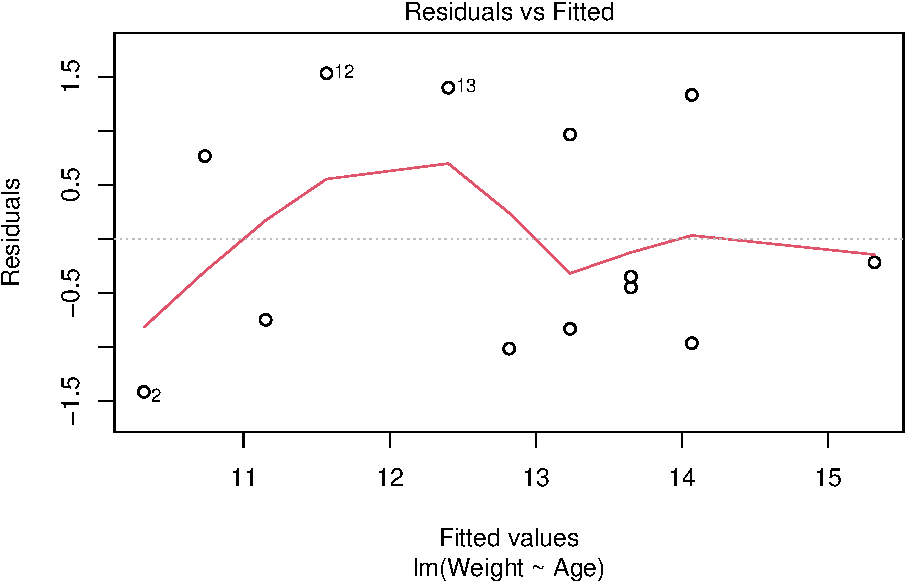
\includegraphics[width=0.5\linewidth]{examples_files/figure-latex/unnamed-chunk-43-1}
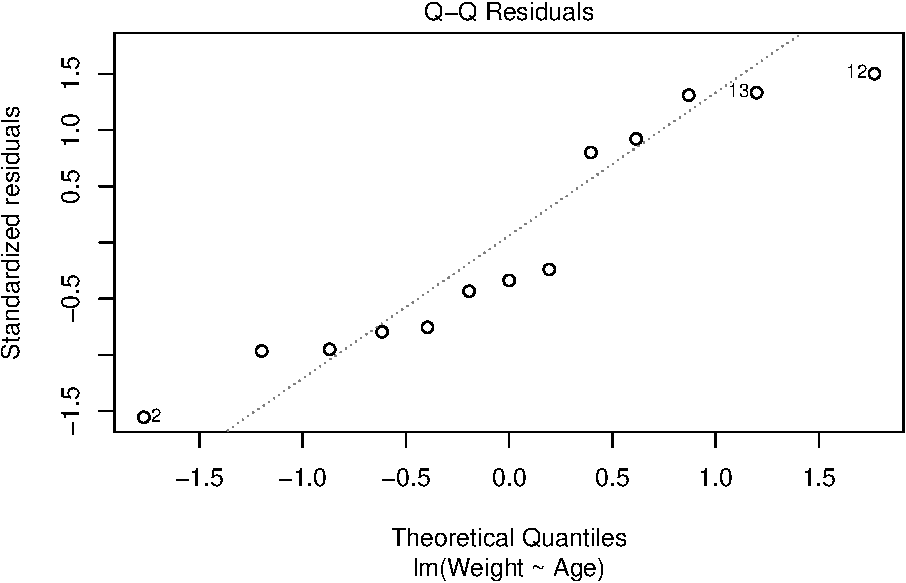
\includegraphics[width=0.5\linewidth]{examples_files/figure-latex/unnamed-chunk-43-2}
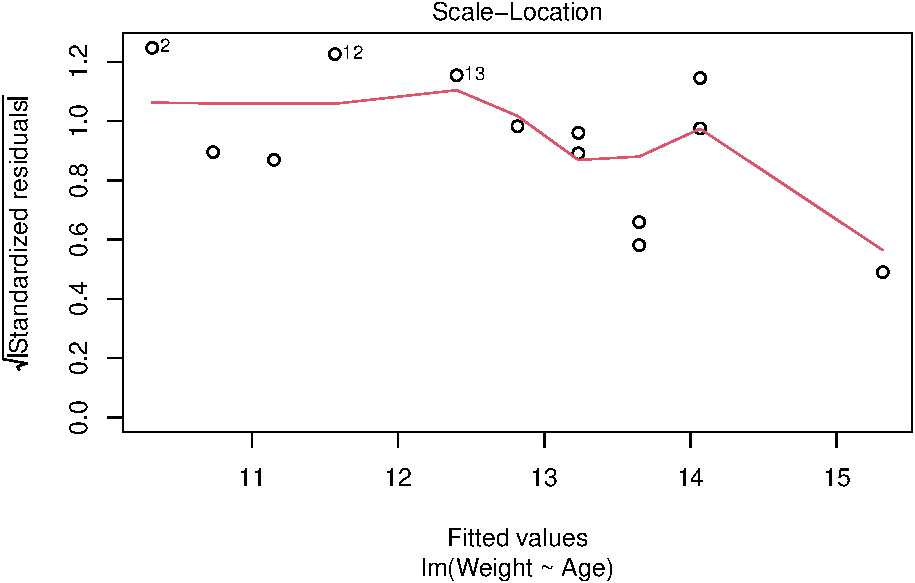
\includegraphics[width=0.5\linewidth]{examples_files/figure-latex/unnamed-chunk-43-3}
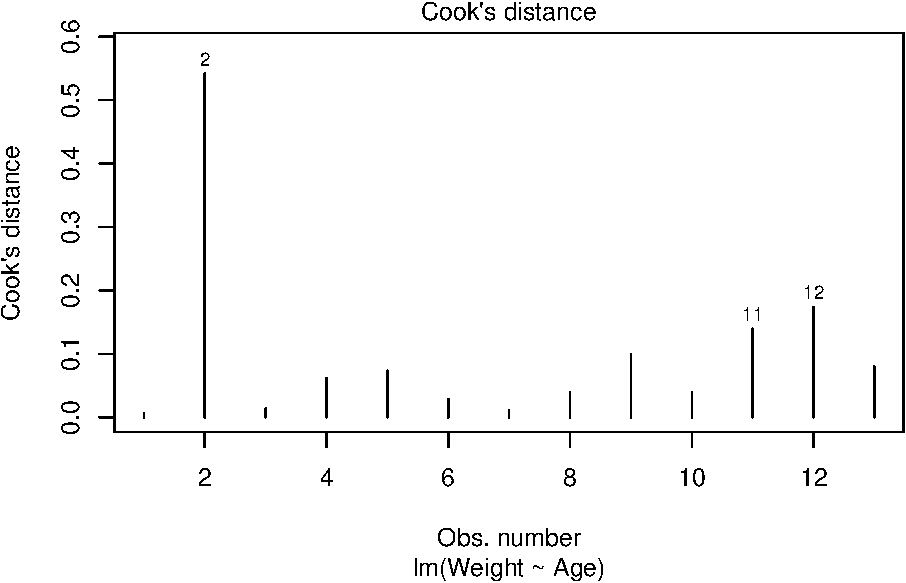
\includegraphics[width=0.5\linewidth]{examples_files/figure-latex/unnamed-chunk-43-4}
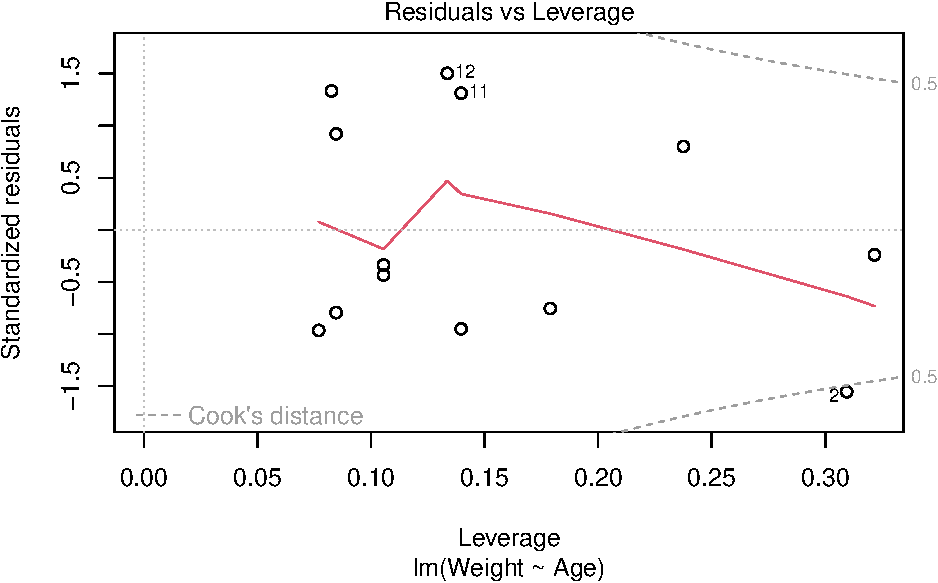
\includegraphics[width=0.5\linewidth]{examples_files/figure-latex/unnamed-chunk-43-5}
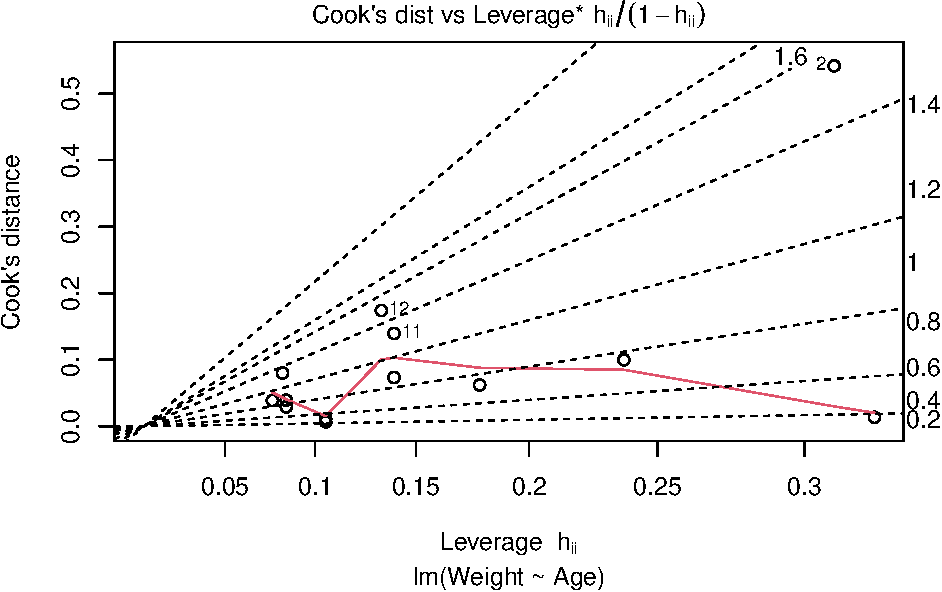
\includegraphics[width=0.5\linewidth]{examples_files/figure-latex/unnamed-chunk-43-6}

We can see from the qq-plot, that the normally assumption of the
residuals may not be reasonable. We can also see from the residuals vs
fitted plot that there is a curve in the data, which tells us that our
linear model may not be a good fit. Using the criteria that an
observation is influential when Cook's distance \(D_i > 1\), we see
there are no influential points.

Now we can try fitting the model with our 2 dummy variables to see if it
improves,

\begin{Shaded}
\begin{Highlighting}[]
\NormalTok{model2 }\OtherTok{\textless{}{-}} \FunctionTok{lm}\NormalTok{(Weight }\SpecialCharTok{\textasciitilde{}}\NormalTok{ Age }\SpecialCharTok{+}\NormalTok{ Z1 }\SpecialCharTok{+}\NormalTok{ Z2, }\AttributeTok{data=}\NormalTok{turkey)}
\FunctionTok{summary}\NormalTok{(model2)}
\end{Highlighting}
\end{Shaded}

\begin{verbatim}
## 
## Call:
## lm(formula = Weight ~ Age + Z1 + Z2, data = turkey)
## 
## Residuals:
##      Min       1Q   Median       3Q      Max 
## -0.37353 -0.15294  0.01103  0.17868  0.47353 
## 
## Coefficients:
##             Estimate Std. Error t value Pr(>|t|)    
## (Intercept)  1.43088    0.65744   2.176   0.0575 .  
## Age          0.48676    0.02574  18.908 1.49e-08 ***
## Z1          -1.91838    0.20180  -9.506 5.45e-06 ***
## Z2          -2.19191    0.21143 -10.367 2.65e-06 ***
## ---
## Signif. codes:  0 '***' 0.001 '**' 0.01 '*' 0.05 '.' 0.1 ' ' 1
## 
## Residual standard error: 0.3002 on 9 degrees of freedom
## Multiple R-squared:  0.9794, Adjusted R-squared:  0.9726 
## F-statistic: 142.8 on 3 and 9 DF,  p-value: 6.6e-08
\end{verbatim}

We see that all the predictors are significant, and our \(R^2\) value
has increased significantly. We can examine the model adequency again,

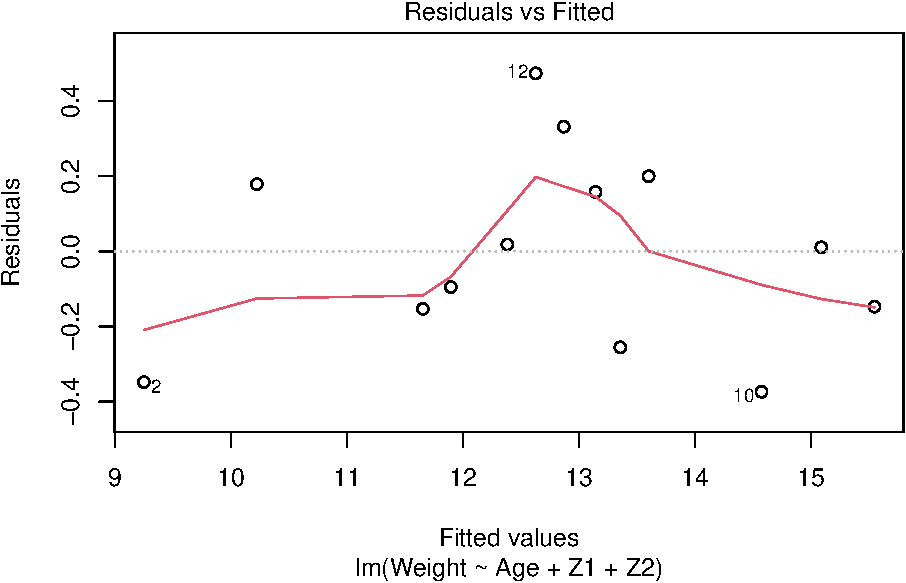
\includegraphics[width=0.5\linewidth]{examples_files/figure-latex/unnamed-chunk-45-1}
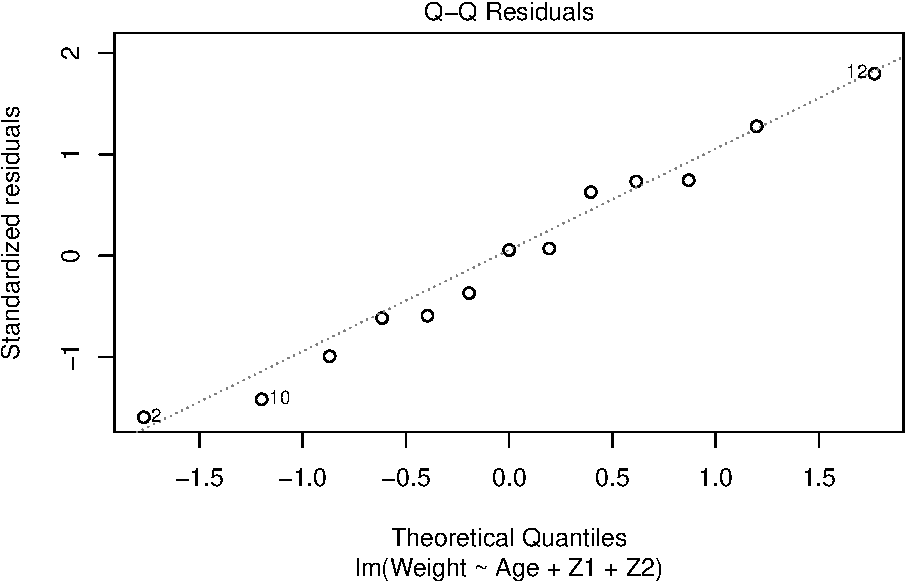
\includegraphics[width=0.5\linewidth]{examples_files/figure-latex/unnamed-chunk-45-2}
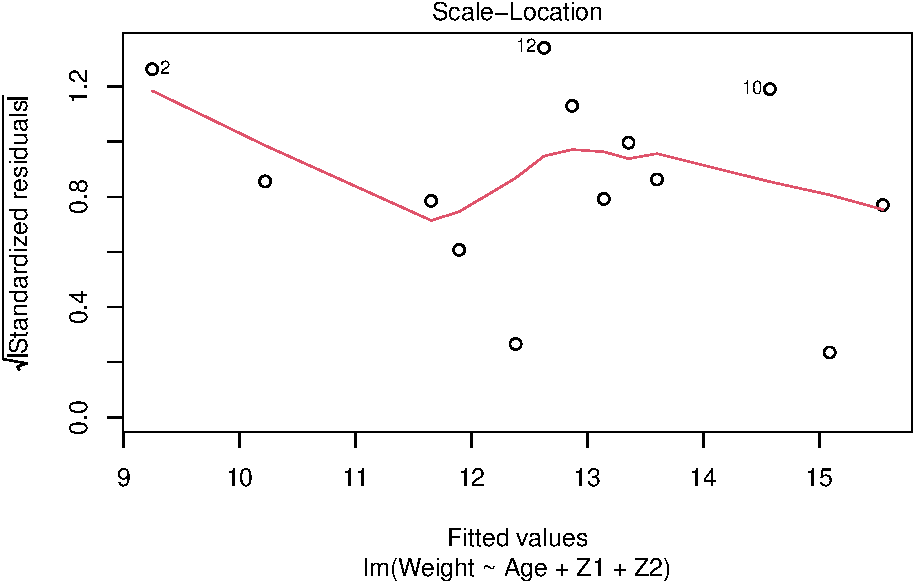
\includegraphics[width=0.5\linewidth]{examples_files/figure-latex/unnamed-chunk-45-3}
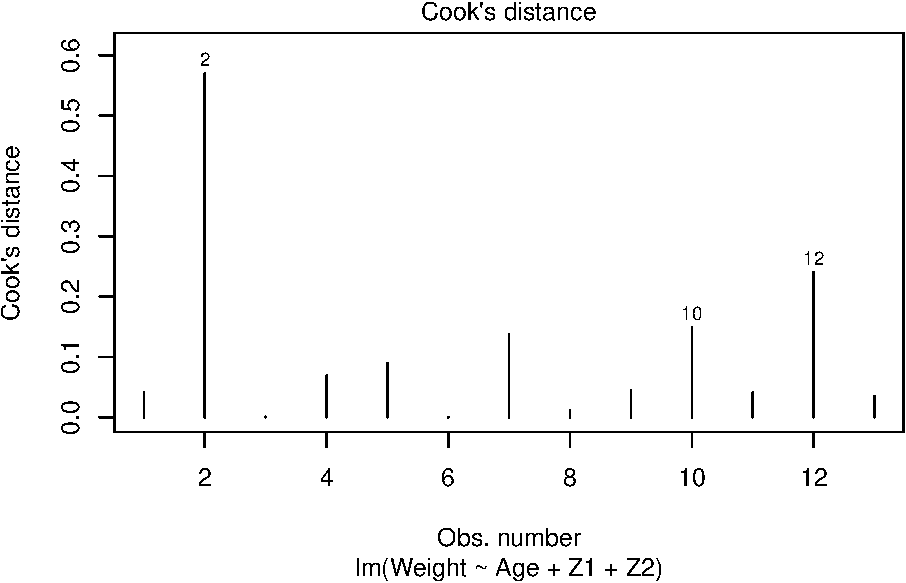
\includegraphics[width=0.5\linewidth]{examples_files/figure-latex/unnamed-chunk-45-4}
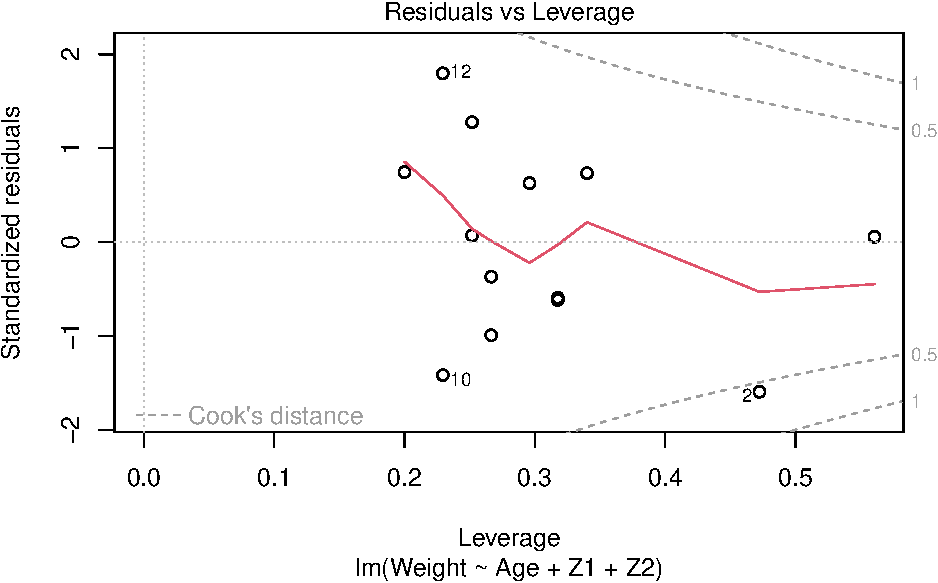
\includegraphics[width=0.5\linewidth]{examples_files/figure-latex/unnamed-chunk-45-5}
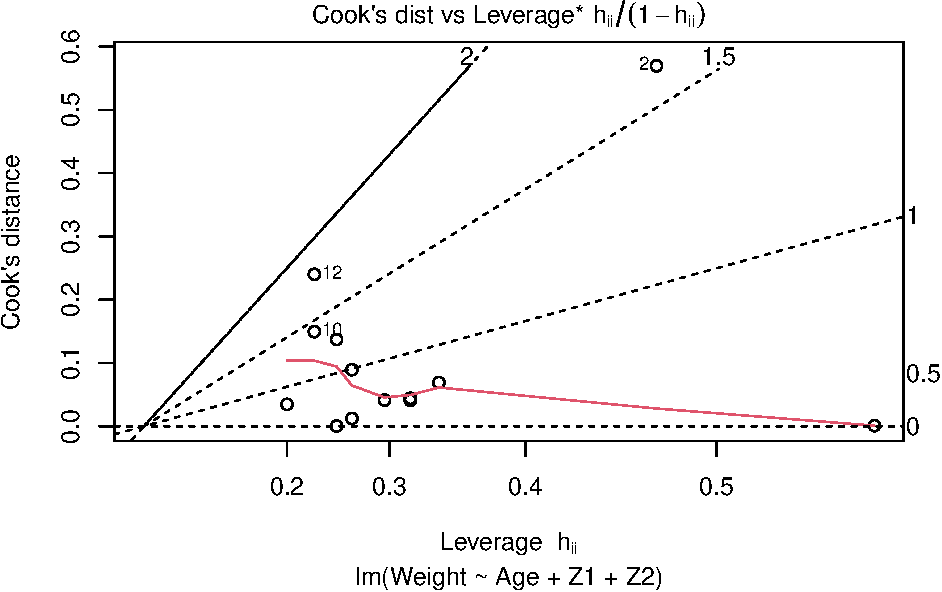
\includegraphics[width=0.5\linewidth]{examples_files/figure-latex/unnamed-chunk-45-6}

The qq-plot shows the assumption of normally distributed residuals is
more reasonable now, and the residuals vs fitted is looking more random,
however there still is a slight curve which could require more
adjustments.

\subsection{Example with Polynomial
Regression}\label{example-with-polynomial-regression}

For this example we will use the hardwood dataset, we'll start by
fitting a simple model and examining its adequecy,

\begin{Shaded}
\begin{Highlighting}[]
\NormalTok{hardwood }\OtherTok{\textless{}{-}} \FunctionTok{read.table}\NormalTok{(}\StringTok{"./Data/hardwood.txt"}\NormalTok{,}\AttributeTok{header=}\ConstantTok{TRUE}\NormalTok{, }\AttributeTok{sep=}\StringTok{\textquotesingle{}}\SpecialCharTok{\textbackslash{}t}\StringTok{\textquotesingle{}}\NormalTok{)}
\NormalTok{x }\OtherTok{\textless{}{-}}\NormalTok{ hardwood}\SpecialCharTok{$}\NormalTok{Concentration}
\NormalTok{y }\OtherTok{\textless{}{-}}\NormalTok{ hardwood}\SpecialCharTok{$}\NormalTok{Tensile.Strength.Y}
\NormalTok{model1 }\OtherTok{\textless{}{-}} \FunctionTok{lm}\NormalTok{(y }\SpecialCharTok{\textasciitilde{}}\NormalTok{ x)}
\FunctionTok{par}\NormalTok{(}\AttributeTok{mfrow=}\FunctionTok{c}\NormalTok{(}\DecValTok{2}\NormalTok{,}\DecValTok{2}\NormalTok{))}
\FunctionTok{plot}\NormalTok{(model1)}
\end{Highlighting}
\end{Shaded}

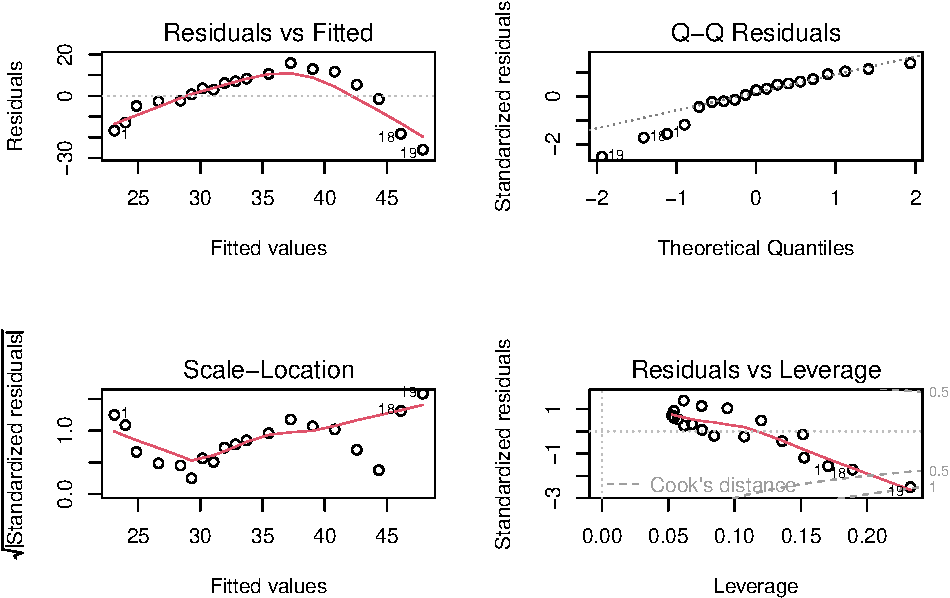
\includegraphics{examples_files/figure-latex/unnamed-chunk-46-1.pdf}

We can see from the residuals vs fitted, a very clear parabola shape is
present, which indicates that there may be a non linear relationship our
model is failing to account for. So, we will try to fit a quadratic
model,

\begin{Shaded}
\begin{Highlighting}[]
\NormalTok{model2 }\OtherTok{\textless{}{-}} \FunctionTok{lm}\NormalTok{(y }\SpecialCharTok{\textasciitilde{}}\NormalTok{ x }\SpecialCharTok{+} \FunctionTok{I}\NormalTok{(x}\SpecialCharTok{\^{}}\DecValTok{2}\NormalTok{))}
\FunctionTok{par}\NormalTok{(}\AttributeTok{mfrow=}\FunctionTok{c}\NormalTok{(}\DecValTok{2}\NormalTok{,}\DecValTok{2}\NormalTok{))}
\FunctionTok{plot}\NormalTok{(model2)}
\end{Highlighting}
\end{Shaded}

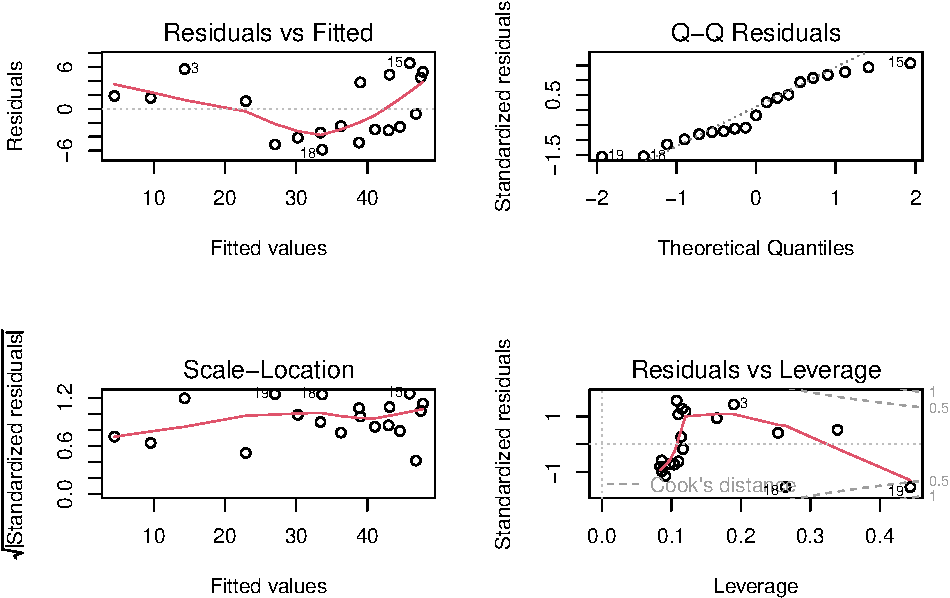
\includegraphics{examples_files/figure-latex/unnamed-chunk-47-1.pdf}

We can see now that the residuals vs fitted is slightly more random,
however there is still a curve which indicates that there is evidence of
a non linear relationship, and that the assumption of constant variance
may not be reasonable. A higher order polynomial may be needed to fit
the data better. We can also examine the differences in the \(R^2\)
values that we get from the 2 models,

\begin{Shaded}
\begin{Highlighting}[]
\FunctionTok{summary}\NormalTok{(model1)}\SpecialCharTok{$}\NormalTok{r.squared}
\end{Highlighting}
\end{Shaded}

\begin{verbatim}
## [1] 0.3053739
\end{verbatim}

\begin{Shaded}
\begin{Highlighting}[]
\FunctionTok{summary}\NormalTok{(model2)}\SpecialCharTok{$}\NormalTok{r.squared}
\end{Highlighting}
\end{Shaded}

\begin{verbatim}
## [1] 0.908502
\end{verbatim}

As we can see, the \(R^2\) value for the quadratic model is much higher,
so we can conclude that the quadratic model is a better fit.

\section{Chapter 8 -
Multicolinearity}\label{chapter-8---multicolinearity}

We will use the acetylene dataset for this example.

\begin{Shaded}
\begin{Highlighting}[]
\NormalTok{acetylene }\OtherTok{\textless{}{-}} \FunctionTok{read.table}\NormalTok{(}\StringTok{"./Data/acetylene.txt"}\NormalTok{,}\AttributeTok{header=}\ConstantTok{TRUE}\NormalTok{, }\AttributeTok{sep=}\StringTok{\textquotesingle{}}\SpecialCharTok{\textbackslash{}t}\StringTok{\textquotesingle{}}\NormalTok{)}
\NormalTok{acetylene}
\end{Highlighting}
\end{Shaded}

\begin{verbatim}
##    Acetylene Temperature Ratio Contact.Time
## 1       49.0        1300   7.5       0.0120
## 2       50.2        1300   9.0       0.0120
## 3       50.5        1300  11.0       0.0115
## 4       48.5        1300  13.5       0.0130
## 5       47.5        1300  17.0       0.0135
## 6       44.5        1300  23.0       0.0120
## 7       28.0        1200   5.3       0.0400
## 8       31.5        1200   7.5       0.0380
## 9       34.5        1200  11.0       0.0320
## 10      35.0        1200  13.5       0.0260
## 11      38.0        1200  17.0       0.0340
## 12      38.5        1200  23.0       0.0410
## 13      15.0        1100   5.3       0.0840
## 14      17.0        1100   7.5       0.0980
## 15      20.5        1100  11.0       0.0920
## 16      29.5        1100  17.0       0.0860
\end{verbatim}

We want to consider the full quadratic model which takes into account
the interactions as well, and we want each of the regression to be
scaled using the unit normal scaling (subtract mean and divide by
standard deviation).

\begin{Shaded}
\begin{Highlighting}[]
\NormalTok{P }\OtherTok{\textless{}{-}}\NormalTok{ acetylene}\SpecialCharTok{$}\NormalTok{Acetylene}
\NormalTok{T }\OtherTok{\textless{}{-}} \FunctionTok{scale}\NormalTok{(acetylene}\SpecialCharTok{$}\NormalTok{Temperature)}
\NormalTok{H }\OtherTok{\textless{}{-}} \FunctionTok{scale}\NormalTok{(acetylene}\SpecialCharTok{$}\NormalTok{Ratio)}
\NormalTok{C }\OtherTok{\textless{}{-}} \FunctionTok{scale}\NormalTok{(acetylene}\SpecialCharTok{$}\NormalTok{Contact.Time)}

\NormalTok{model }\OtherTok{\textless{}{-}} \FunctionTok{lm}\NormalTok{(P }\SpecialCharTok{\textasciitilde{}}\NormalTok{ T }\SpecialCharTok{+}\NormalTok{ H }\SpecialCharTok{+}\NormalTok{ C }\SpecialCharTok{+} \FunctionTok{I}\NormalTok{(T}\SpecialCharTok{\^{}}\DecValTok{2}\NormalTok{) }\SpecialCharTok{+} \FunctionTok{I}\NormalTok{(H}\SpecialCharTok{\^{}}\DecValTok{2}\NormalTok{) }\SpecialCharTok{+} \FunctionTok{I}\NormalTok{(C}\SpecialCharTok{\^{}}\DecValTok{2}\NormalTok{) }\SpecialCharTok{+}\NormalTok{ T}\SpecialCharTok{*}\NormalTok{H }\SpecialCharTok{+}\NormalTok{ T}\SpecialCharTok{*}\NormalTok{C }\SpecialCharTok{+}\NormalTok{ H}\SpecialCharTok{*}\NormalTok{C)}
\FunctionTok{summary}\NormalTok{(model)}
\end{Highlighting}
\end{Shaded}

\begin{verbatim}
## 
## Call:
## lm(formula = P ~ T + H + C + I(T^2) + I(H^2) + I(C^2) + T * H + 
##     T * C + H * C)
## 
## Residuals:
##     Min      1Q  Median      3Q     Max 
## -1.3499 -0.3411  0.1297  0.5011  0.6720 
## 
## Coefficients:
##             Estimate Std. Error t value Pr(>|t|)    
## (Intercept)  35.8958     1.0916  32.884 5.26e-08 ***
## T             4.0038     4.5087   0.888 0.408719    
## H             2.7783     0.3071   9.048 0.000102 ***
## C            -8.0423     6.0707  -1.325 0.233461    
## I(T^2)      -12.5236    12.3238  -1.016 0.348741    
## I(H^2)       -0.9727     0.3746  -2.597 0.040844 *  
## I(C^2)      -11.5932     7.7063  -1.504 0.183182    
## T:H          -6.4568     1.4660  -4.404 0.004547 ** 
## T:C         -26.9804    21.0213  -1.283 0.246663    
## H:C          -3.7681     1.6553  -2.276 0.063116 .  
## ---
## Signif. codes:  0 '***' 0.001 '**' 0.01 '*' 0.05 '.' 0.1 ' ' 1
## 
## Residual standard error: 0.9014 on 6 degrees of freedom
## Multiple R-squared:  0.9977, Adjusted R-squared:  0.9943 
## F-statistic: 289.7 on 9 and 6 DF,  p-value: 3.225e-07
\end{verbatim}

This gives us our model

\[\hat{P} = 35.8958 + 4.0038T + 2.7783 H -8.0423C -6.4568TH -26.9804TC\]
\[-3.7681HC -12.5236T^2 -0.9727H^2-11.5932C^2\]

We can examine the correlation between our predictors

\begin{Shaded}
\begin{Highlighting}[]
\NormalTok{predictors }\OtherTok{\textless{}{-}} \FunctionTok{c}\NormalTok{(T,H,C, T}\SpecialCharTok{*}\NormalTok{H, T}\SpecialCharTok{*}\NormalTok{C, H}\SpecialCharTok{*}\NormalTok{C, T}\SpecialCharTok{\^{}}\DecValTok{2}\NormalTok{, H}\SpecialCharTok{\^{}}\DecValTok{2}\NormalTok{, C}\SpecialCharTok{\^{}}\DecValTok{2}\NormalTok{)}

\NormalTok{df }\OtherTok{\textless{}{-}} \FunctionTok{data.frame}\NormalTok{(T, H, C, T}\SpecialCharTok{*}\NormalTok{H, H}\SpecialCharTok{*}\NormalTok{C, T}\SpecialCharTok{*}\NormalTok{C, T}\SpecialCharTok{\^{}}\DecValTok{2}\NormalTok{, H}\SpecialCharTok{\^{}}\DecValTok{2}\NormalTok{, C}\SpecialCharTok{\^{}}\DecValTok{2}\NormalTok{)}
\FunctionTok{round}\NormalTok{(}\FunctionTok{cor}\NormalTok{(df), }\DecValTok{3}\NormalTok{)}
\end{Highlighting}
\end{Shaded}

\begin{verbatim}
##            T      H      C  T...H  H...C  T...C    T.2    H.2    C.2
## T      1.000  0.224 -0.958 -0.132  0.206  0.443 -0.271  0.031 -0.577
## H      0.224  1.000 -0.240  0.039 -0.023  0.192 -0.148  0.498 -0.224
## C     -0.958 -0.240  1.000  0.195 -0.274 -0.661  0.501 -0.018  0.765
## T...H -0.132  0.039  0.195  1.000 -0.974 -0.265  0.246  0.398  0.275
## H...C  0.206 -0.023 -0.274 -0.974  1.000  0.324 -0.279 -0.375 -0.359
## T...C  0.443  0.192 -0.661 -0.265  0.324  1.000 -0.972  0.126 -0.972
## T.2   -0.271 -0.148  0.501  0.246 -0.279 -0.972  1.000 -0.124  0.894
## H.2    0.031  0.498 -0.018  0.398 -0.375  0.126 -0.124  1.000 -0.158
## C.2   -0.577 -0.224  0.765  0.275 -0.359 -0.972  0.894 -0.158  1.000
\end{verbatim}

As we can see, there's high correlation between temperataure and contact
time, and there are other large correlations between \(x_1x_2\) and
\(x_2x_3\), \(x_1x_3\) and \(x_1^2\), and \(x_1^2\) and \(x_3^3\). This
is not surprising since these variables are generated from the linear
terms and involve highly correlated regressors \(x_1\) and \(x_3\).

We can compute the variance inflation factors for each of the
predictors,

\begin{Shaded}
\begin{Highlighting}[]
\FunctionTok{library}\NormalTok{(car)}
\FunctionTok{vif}\NormalTok{(model)}
\end{Highlighting}
\end{Shaded}

\begin{verbatim}
##           T           H           C      I(T^2)      I(H^2)      I(C^2) 
##  375.247759    1.740631  680.280039 1762.575365    3.164318 1156.766284 
##         T:H         T:C         H:C 
##   31.037059 6563.345193   35.611286
\end{verbatim}

As we can see many of these have very high VIF, which certainly
indicates multicollinearity. We can also compute the condition number
\(\kappa\) and condition indices
\(\kappa_j = \frac{\lambda_{\max}}{\lambda_j}\). Note that \(\lambda_j\)
are the eigenvalues for the matrix \(X'X\).

\begin{Shaded}
\begin{Highlighting}[]
\NormalTok{eigen\_values }\OtherTok{\textless{}{-}} \FunctionTok{eigen}\NormalTok{(}\FunctionTok{cor}\NormalTok{(df))}\SpecialCharTok{$}\NormalTok{values}
\NormalTok{eigen\_values}
\end{Highlighting}
\end{Shaded}

\begin{verbatim}
## [1] 4.205230e+00 2.161999e+00 1.138677e+00 1.040475e+00 3.852305e-01
## [6] 4.953807e-02 1.362526e-02 5.127803e-03 9.693644e-05
\end{verbatim}

\begin{Shaded}
\begin{Highlighting}[]
\NormalTok{kappa }\OtherTok{\textless{}{-}} \FunctionTok{max}\NormalTok{(eigen\_values) }\SpecialCharTok{/} \FunctionTok{min}\NormalTok{(eigen\_values)}
\NormalTok{kappa}
\end{Highlighting}
\end{Shaded}

\begin{verbatim}
## [1] 43381.31
\end{verbatim}

\begin{Shaded}
\begin{Highlighting}[]
\NormalTok{kappa\_j }\OtherTok{\textless{}{-}} \FunctionTok{max}\NormalTok{(eigen\_values) }\SpecialCharTok{/}\NormalTok{ eigen\_values}
\NormalTok{kappa\_j}
\end{Highlighting}
\end{Shaded}

\begin{verbatim}
## [1]     1.000000     1.945066     3.693085     4.041644    10.916141
## [6]    84.888858   308.634770   820.084287 43381.314197
\end{verbatim}

As we can see, the condition number \(\kappa = 43381.31\) is very large
which indicates severe multicollinearity. The condition indices greater
than 1000 indicate severe multicollinearity, those between 100 and 1000
indicate moderate to strong multicollinearity, and those bellow 100 have
no indication of multicollinearity.

We can compute the tolerance values as well

\begin{Shaded}
\begin{Highlighting}[]
\FunctionTok{ols\_coll\_diag}\NormalTok{(model)}\SpecialCharTok{$}\NormalTok{vif\_t}
\end{Highlighting}
\end{Shaded}

\begin{verbatim}
##   Variables    Tolerance         VIF
## 1         T 0.0026649060  375.247759
## 2         H 0.5745042909    1.740631
## 3         C 0.0014699829  680.280039
## 4    I(T^2) 0.0005673516 1762.575365
## 5    I(H^2) 0.3160238460    3.164318
## 6    I(C^2) 0.0008644789 1156.766284
## 7       T:H 0.0322195480   31.037059
## 8       T:C 0.0001523613 6563.345193
## 9       H:C 0.0280809849   35.611286
\end{verbatim}

Tolerance is the amount of variability in one independent variable that
is not explained by the other independent variables. To compute it,
regress the \(k\)th predictor on the other predictors in the model and
compute the \(R^2\) value, then Tolerance \(= 1- R^2\). Tolerance values
less than 0.10 indicate collinearity.

We can preform ridge regression now as well

\begin{Shaded}
\begin{Highlighting}[]
\NormalTok{ridge\_model }\OtherTok{\textless{}{-}} \FunctionTok{lm.ridge}\NormalTok{(P }\SpecialCharTok{\textasciitilde{}}\NormalTok{ T }\SpecialCharTok{+}\NormalTok{ H }\SpecialCharTok{+}\NormalTok{ C }\SpecialCharTok{+} \FunctionTok{I}\NormalTok{(T}\SpecialCharTok{\^{}}\DecValTok{2}\NormalTok{) }\SpecialCharTok{+} \FunctionTok{I}\NormalTok{(H}\SpecialCharTok{\^{}}\DecValTok{2}\NormalTok{) }\SpecialCharTok{+} \FunctionTok{I}\NormalTok{(C}\SpecialCharTok{\^{}}\DecValTok{2}\NormalTok{)}
                        \SpecialCharTok{+}\NormalTok{ T}\SpecialCharTok{*}\NormalTok{H }\SpecialCharTok{+}\NormalTok{ T}\SpecialCharTok{*}\NormalTok{C }\SpecialCharTok{+}\NormalTok{ H}\SpecialCharTok{*}\NormalTok{C, }\AttributeTok{lambda=}\FunctionTok{seq}\NormalTok{(}\DecValTok{0}\NormalTok{,}\FloatTok{0.1}\NormalTok{,}\FloatTok{0.01}\NormalTok{))}
\FunctionTok{plot}\NormalTok{(ridge\_model)}
\end{Highlighting}
\end{Shaded}

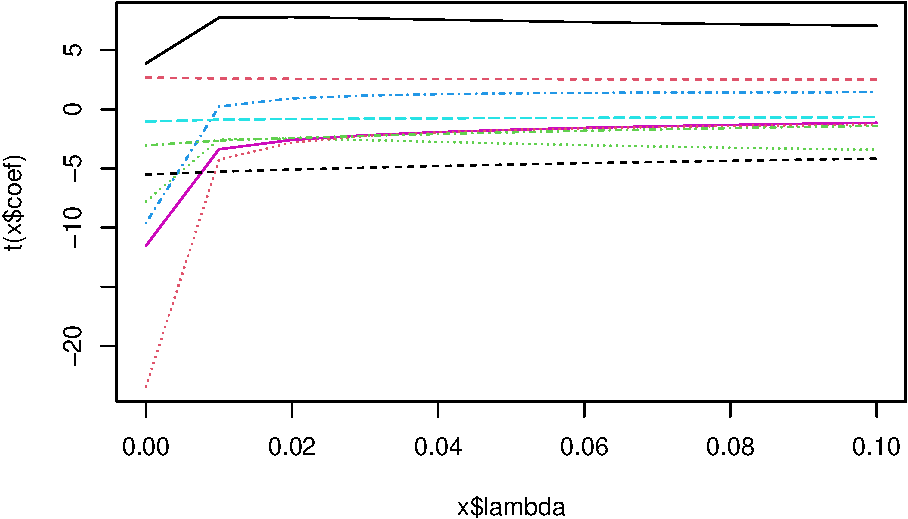
\includegraphics{examples_files/figure-latex/unnamed-chunk-55-1.pdf}

The y axis represents the coefficient \(\hat{\beta}_R\) which is the
solution to the equation \((X'X + cI)\hat{\beta}_R = X'Y\), the x-axis
is those values of \(c\) that we are looking for. We want to choose
\(c\) large enough to provide stable coefficients but not too large. Now
we want to preform cross validation and obtain the best value for \(c\).

\begin{Shaded}
\begin{Highlighting}[]
\FunctionTok{library}\NormalTok{(glmnet)}

\NormalTok{x }\OtherTok{=} \FunctionTok{data.matrix}\NormalTok{(df)}
\NormalTok{y }\OtherTok{=}\NormalTok{ P}
\NormalTok{model }\OtherTok{\textless{}{-}} \FunctionTok{glmnet}\NormalTok{(x,y, }\AttributeTok{alpha=}\DecValTok{0}\NormalTok{)}
\NormalTok{cv\_model }\OtherTok{\textless{}{-}} \FunctionTok{cv.glmnet}\NormalTok{(x,y, }\AttributeTok{alpha=}\DecValTok{0}\NormalTok{)}
\FunctionTok{plot}\NormalTok{(cv\_model)}
\end{Highlighting}
\end{Shaded}

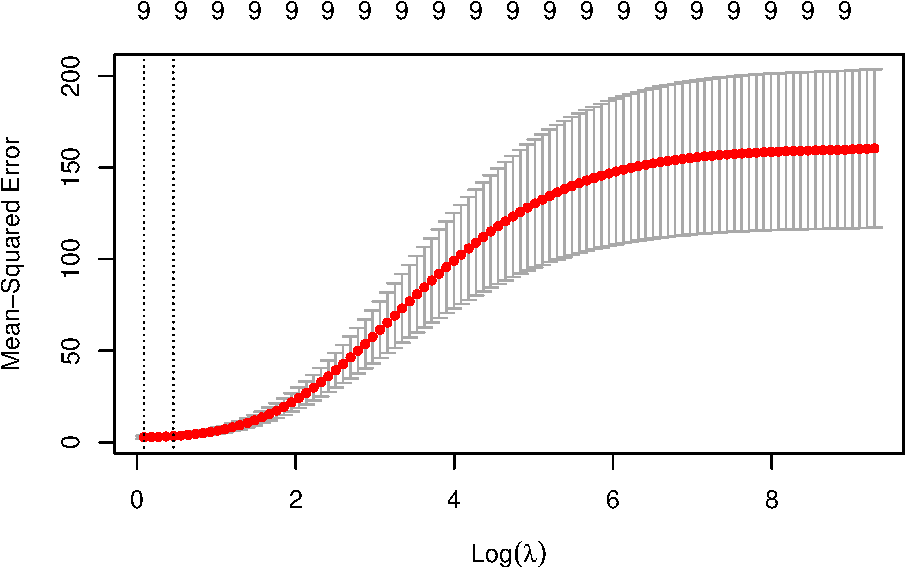
\includegraphics{examples_files/figure-latex/unnamed-chunk-56-1.pdf}

Now we can extract the optimal value of lambda and create the best
model,

\begin{Shaded}
\begin{Highlighting}[]
\NormalTok{lambda }\OtherTok{\textless{}{-}}\NormalTok{ cv\_model}\SpecialCharTok{$}\NormalTok{lambda.min}
\NormalTok{ridge\_model }\OtherTok{\textless{}{-}} \FunctionTok{glmnet}\NormalTok{(x,y, }\AttributeTok{alpha=}\DecValTok{0}\NormalTok{, }\AttributeTok{lambda=}\NormalTok{lambda)}
\FunctionTok{coef}\NormalTok{(ridge\_model)}
\end{Highlighting}
\end{Shaded}

\begin{verbatim}
## 10 x 1 sparse Matrix of class "dgCMatrix"
##                     s0
## (Intercept) 35.2178148
## T            5.8931581
## H            2.4034813
## C           -4.4901599
## T...H       -2.2227495
## H...C        1.0499186
## T...C       -0.6879354
## T.2          1.8762583
## H.2         -0.4899215
## C.2         -0.3485636
\end{verbatim}

\section{Chapter 9 - Model Selection}\label{chapter-9---model-selection}

We will use the Hald Cement dataset for this example.

\begin{Shaded}
\begin{Highlighting}[]
\NormalTok{cement }\OtherTok{\textless{}{-}} \FunctionTok{read.table}\NormalTok{(}\StringTok{"./Data/cement.txt"}\NormalTok{,}\AttributeTok{header=}\ConstantTok{TRUE}\NormalTok{, }\AttributeTok{sep=}\StringTok{\textquotesingle{}}\SpecialCharTok{\textbackslash{}t}\StringTok{\textquotesingle{}}\NormalTok{)}
\FunctionTok{plot}\NormalTok{(cement)}
\end{Highlighting}
\end{Shaded}

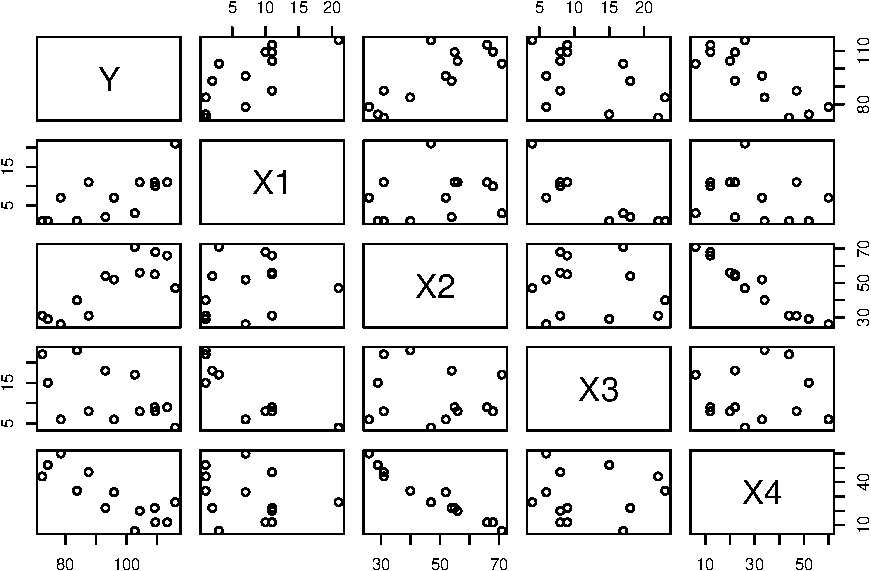
\includegraphics{examples_files/figure-latex/unnamed-chunk-58-1.pdf}

Looking at the scatterplots, we can see there may be some
multicollinearity between \(X_2\) and \(X_4\). Examining this further we
find

\begin{Shaded}
\begin{Highlighting}[]
\FunctionTok{cor}\NormalTok{(cement)}
\end{Highlighting}
\end{Shaded}

\begin{verbatim}
##             Y         X1         X2         X3         X4
## Y   1.0000000  0.7307175  0.8162526 -0.5346707 -0.8213050
## X1  0.7307175  1.0000000  0.2285795 -0.8241338 -0.2454451
## X2  0.8162526  0.2285795  1.0000000 -0.1392424 -0.9729550
## X3 -0.5346707 -0.8241338 -0.1392424  1.0000000  0.0295370
## X4 -0.8213050 -0.2454451 -0.9729550  0.0295370  1.0000000
\end{verbatim}

\begin{Shaded}
\begin{Highlighting}[]
\NormalTok{model }\OtherTok{\textless{}{-}} \FunctionTok{lm}\NormalTok{(Y }\SpecialCharTok{\textasciitilde{}}\NormalTok{ X1 }\SpecialCharTok{+}\NormalTok{ X2 }\SpecialCharTok{+}\NormalTok{ X3 }\SpecialCharTok{+}\NormalTok{ X4, }\AttributeTok{data=}\NormalTok{cement)}
\FunctionTok{ols\_coll\_diag}\NormalTok{(model)}\SpecialCharTok{$}\NormalTok{vif\_t}
\end{Highlighting}
\end{Shaded}

\begin{verbatim}
##   Variables   Tolerance       VIF
## 1        X1 0.025976582  38.49621
## 2        X2 0.003930460 254.42317
## 3        X3 0.021336344  46.86839
## 4        X4 0.003539662 282.51286
\end{verbatim}

We can see that there is severe multicollinearity between \(X_2\) and
\(X_4\) and shown by the tolerance being less than 0.1 for both, as well
as a very large VIF. We can also see that \(X_1\) and \(X_3\) have a
large correlation and also high VIF and low tolerance.

This suggests we want to try models that do not include all the
predictotrs. We first try all possible regressions,

\begin{Shaded}
\begin{Highlighting}[]
\FunctionTok{ols\_step\_all\_possible}\NormalTok{(model)}
\end{Highlighting}
\end{Shaded}

\begin{verbatim}
##    Index N  Predictors  R-Square Adj. R-Square Mallow's Cp
## 4      1 1          X4 0.6745420     0.6449549  138.730833
## 2      2 1          X2 0.6662683     0.6359290  142.486407
## 1      3 1          X1 0.5339480     0.4915797  202.548769
## 3      4 1          X3 0.2858727     0.2209521  315.154284
## 5      5 2       X1 X2 0.9786784     0.9744140    2.678242
## 7      6 2       X1 X4 0.9724710     0.9669653    5.495851
## 10     7 2       X3 X4 0.9352896     0.9223476   22.373112
## 8      8 2       X2 X3 0.8470254     0.8164305   62.437716
## 9      9 2       X2 X4 0.6800604     0.6160725  138.225920
## 6     10 2       X1 X3 0.5481667     0.4578001  198.094653
## 12    11 3    X1 X2 X4 0.9823355     0.9764473    3.018233
## 11    12 3    X1 X2 X3 0.9822847     0.9763796    3.041280
## 13    13 3    X1 X3 X4 0.9812811     0.9750415    3.496824
## 14    14 3    X2 X3 X4 0.9728200     0.9637599    7.337474
## 15    15 4 X1 X2 X3 X4 0.9823756     0.9735634    5.000000
\end{verbatim}

We can see that the model with 3 predictors \(X_1\),\(X_2\), and \(X_4\)
has the \(C_p\) value closest to the number of predictors, as well as
one of the highest \(R^2\) values. However, we know there is strong
multicollinearity between \(X_2\) and \(X_4\), and the model with
\(X_1\), \(X_2\) and \(X_3\) had a slightly higher \(C_p\) value and a
similar \(R^2\). But, we run into the same issue since we know \(X_1\)
and \(X_3\) have multicollinearity, so the next best option would be the
model with only \(X_1\) and \(X_2\). It has a lower \(R^2\) value but it
is still very high at 0.979, and the \(C_p\) value is 2.67 which is also
close to the number of predictors. So, we will select the model with
\(X_1\) and \(X_2\).

Now using best subset selection,

\begin{Shaded}
\begin{Highlighting}[]
\FunctionTok{ols\_step\_best\_subset}\NormalTok{(model)}
\end{Highlighting}
\end{Shaded}

\begin{verbatim}
##  Best Subsets Regression  
## --------------------------
## Model Index    Predictors
## --------------------------
##      1         X4          
##      2         X1 X2       
##      3         X1 X2 X4    
##      4         X1 X2 X3 X4 
## --------------------------
## 
##                                                     Subsets Regression Summary                                                    
## ----------------------------------------------------------------------------------------------------------------------------------
##                        Adj.        Pred                                                                                            
## Model    R-Square    R-Square    R-Square      C(p)        AIC       SBIC        SBC        MSEP         FPE       HSP       APC  
## ----------------------------------------------------------------------------------------------------------------------------------
##   1        0.6745      0.6450      0.5603    138.7308    97.7440    55.5401    99.4389    1047.0423    92.7133    8.0352    0.4438 
##   2        0.9787      0.9744      0.9654      2.6782    64.3124    29.2437    66.5722      76.2162     7.1267    0.6434    0.0341 
##   3        0.9823      0.9764      0.9686      3.0182    63.8663    31.1723    66.6910      71.0365     6.9704    0.6663    0.0334 
##   4        0.9824      0.9736      0.9594      5.0000    65.8367    34.4130    69.2264      81.0000     8.2841    0.8547    0.0397 
## ----------------------------------------------------------------------------------------------------------------------------------
## AIC: Akaike Information Criteria 
##  SBIC: Sawa's Bayesian Information Criteria 
##  SBC: Schwarz Bayesian Criteria 
##  MSEP: Estimated error of prediction, assuming multivariate normality 
##  FPE: Final Prediction Error 
##  HSP: Hocking's Sp 
##  APC: Amemiya Prediction Criteria
\end{verbatim}

We can see that the best model in terms of the \(C_p\) statistic and the
\(R^2\) value is again the model with \(X_1, X_2\) and \(X_4\). But, as
we previously mentioned this model suffers from multicollinearity due to
\(X_2\) and \(X_4\) being present. So, we pick the second best model
which is \(X_1\) and \(X_2\) again.

Now using forward selection,

\begin{Shaded}
\begin{Highlighting}[]
\FunctionTok{ols\_step\_forward\_p}\NormalTok{(model)}
\end{Highlighting}
\end{Shaded}

\begin{verbatim}
## 
##                             Selection Summary                             
## -------------------------------------------------------------------------
##         Variable                  Adj.                                       
## Step    Entered     R-Square    R-Square      C(p)        AIC       RMSE     
## -------------------------------------------------------------------------
##    1    X4            0.6745      0.6450    138.7308    97.7440    8.9639    
##    2    X1            0.9725      0.9670      5.4959    67.6341    2.7343    
##    3    X2            0.9823      0.9764      3.0182    63.8663    2.3087    
## -------------------------------------------------------------------------
\end{verbatim}

We can see that first \(X_4\) was entered, then \(X_1\), then \(X_2\)
resulting in the same model that we saw was the best in the previous 2
methods. However, selecting this model would lead to multicollinearity
as we've discussed.

With backwards elimination,

\begin{Shaded}
\begin{Highlighting}[]
\FunctionTok{ols\_step\_backward\_p}\NormalTok{(model)}
\end{Highlighting}
\end{Shaded}

\begin{verbatim}
## 
## 
##                           Elimination Summary                           
## -----------------------------------------------------------------------
##         Variable                  Adj.                                     
## Step    Removed     R-Square    R-Square     C(p)       AIC       RMSE     
## -----------------------------------------------------------------------
##    1    X3            0.9823      0.9764    3.0182    63.8663    2.3087    
## -----------------------------------------------------------------------
\end{verbatim}

We can see that we only removed \(X_3\), giving us the same model again
\(X_1\), \(X_2\) and \(X_3\).

Now using stepwise selection,

\begin{Shaded}
\begin{Highlighting}[]
\FunctionTok{ols\_step\_both\_p}\NormalTok{(model)}
\end{Highlighting}
\end{Shaded}

\begin{verbatim}
## 
##                              Stepwise Selection Summary                               
## -------------------------------------------------------------------------------------
##                      Added/                   Adj.                                       
## Step    Variable    Removed     R-Square    R-Square      C(p)        AIC       RMSE     
## -------------------------------------------------------------------------------------
##    1       X4       addition       0.675       0.645    138.7310    97.7440    8.9639    
##    2       X1       addition       0.972       0.967      5.4960    67.6341    2.7343    
##    3       X2       addition       0.982       0.976      3.0180    63.8663    2.3087    
## -------------------------------------------------------------------------------------
\end{verbatim}

Once again, we end up with \(X_1,X_2\) and \(X_4\).

\section{Chapter 10 - Logistic Regression and
GLM's}\label{chapter-10---logistic-regression-and-glms}

\subsection{Example of Logistic
Regression}\label{example-of-logistic-regression}

We'll fit a logistic regression model to the prgoramming experience
dataset.

\begin{Shaded}
\begin{Highlighting}[]
\NormalTok{experience }\OtherTok{\textless{}{-}} \FunctionTok{read.table}\NormalTok{(}\StringTok{"./Data/experience.txt"}\NormalTok{,}\AttributeTok{header=}\ConstantTok{TRUE}\NormalTok{, }\AttributeTok{sep=}\StringTok{\textquotesingle{}}\SpecialCharTok{\textbackslash{}t}\StringTok{\textquotesingle{}}\NormalTok{)}

\NormalTok{mlogit }\OtherTok{\textless{}{-}} \FunctionTok{glm}\NormalTok{(Success }\SpecialCharTok{\textasciitilde{}}\NormalTok{ Experience, }\AttributeTok{data=}\NormalTok{experience, }\AttributeTok{family=}\StringTok{"binomial"}\NormalTok{)}
\FunctionTok{summary}\NormalTok{(mlogit)}
\end{Highlighting}
\end{Shaded}

\begin{verbatim}
## 
## Call:
## glm(formula = Success ~ Experience, family = "binomial", data = experience)
## 
## Coefficients:
##             Estimate Std. Error z value Pr(>|z|)  
## (Intercept) -3.05970    1.25935  -2.430   0.0151 *
## Experience   0.16149    0.06498   2.485   0.0129 *
## ---
## Signif. codes:  0 '***' 0.001 '**' 0.01 '*' 0.05 '.' 0.1 ' ' 1
## 
## (Dispersion parameter for binomial family taken to be 1)
## 
##     Null deviance: 34.296  on 24  degrees of freedom
## Residual deviance: 25.425  on 23  degrees of freedom
## AIC: 29.425
## 
## Number of Fisher Scoring iterations: 4
\end{verbatim}

We can see from the summary that our equation for our logistic
regression model

\[\hat{\pi} = \frac{\exp(-3.05970 + 0.16149X_i)}{1 + \exp(-3.05970 + 0.16149X_i)}\]

And we conclude that the regression is significant so we reject the null
hypothesis \(H_0: \beta_1 = 0\). We can compute the confidence intervals
using

\[\hat{\beta}_j \pm z_{\alpha/2} se(\hat{\beta}_j)\] We can find the
\(z\) value with

\begin{Shaded}
\begin{Highlighting}[]
\FunctionTok{qnorm}\NormalTok{(}\FloatTok{0.025}\NormalTok{, }\AttributeTok{lower.tail=}\ConstantTok{FALSE}\NormalTok{)}
\end{Highlighting}
\end{Shaded}

\begin{verbatim}
## [1] 1.959964
\end{verbatim}

So the confidence intervals are

\[-3.05970 \pm 1.960 \cdot 1.25935 = (-5.528026, -0.591374)\]

\[0.16149 \pm 1.960 \cdot 0.06498 = (0.0341292, 0.2888508)\]

\begin{Shaded}
\begin{Highlighting}[]
\FunctionTok{confint.default}\NormalTok{(mlogit)}
\end{Highlighting}
\end{Shaded}

\begin{verbatim}
##                   2.5 %     97.5 %
## (Intercept) -5.52797622 -0.5914155
## Experience   0.03412744  0.2888444
\end{verbatim}

As we can see we get the same outputs in R (slightly off due to
inaccuracy from lookup table).

We can also construct a confidence interval on the odds ratio, with
(e\^{}\{0.0341292\}, e\^{}\{0.2888508\}),

\begin{Shaded}
\begin{Highlighting}[]
\FunctionTok{exp}\NormalTok{(}\FloatTok{0.0341292}\NormalTok{)}
\end{Highlighting}
\end{Shaded}

\begin{verbatim}
## [1] 1.034718
\end{verbatim}

\begin{Shaded}
\begin{Highlighting}[]
\FunctionTok{exp}\NormalTok{(}\FloatTok{0.2888508}\NormalTok{)}
\end{Highlighting}
\end{Shaded}

\begin{verbatim}
## [1] 1.334893
\end{verbatim}

\begin{Shaded}
\begin{Highlighting}[]
\FunctionTok{exp}\NormalTok{(}\FunctionTok{cbind}\NormalTok{(}\AttributeTok{OR =} \FunctionTok{coef}\NormalTok{(mlogit), }\FunctionTok{confint.default}\NormalTok{(mlogit)))}
\end{Highlighting}
\end{Shaded}

\begin{verbatim}
##                     OR       2.5 %    97.5 %
## (Intercept) 0.04690196 0.003974024 0.5535432
## Experience  1.17525591 1.034716464 1.3348840
\end{verbatim}

As we can see we obtain the same answer of (1.035, 1.335) for the
confidence interval on the odds ratio.

\subsection{Example of Poisson
Regression}\label{example-of-poisson-regression}

We will use the aircraft damage dataset for this example and fit a
Poisson regression model.

\begin{Shaded}
\begin{Highlighting}[]
\NormalTok{aircraft }\OtherTok{\textless{}{-}} \FunctionTok{read.table}\NormalTok{(}\StringTok{"./Data/aircraft.txt"}\NormalTok{,}\AttributeTok{header=}\ConstantTok{TRUE}\NormalTok{, }\AttributeTok{sep=}\StringTok{\textquotesingle{}}\SpecialCharTok{\textbackslash{}t}\StringTok{\textquotesingle{}}\NormalTok{)}
\NormalTok{model }\OtherTok{\textless{}{-}} \FunctionTok{glm}\NormalTok{(Y }\SpecialCharTok{\textasciitilde{}}\NormalTok{ X1 }\SpecialCharTok{+}\NormalTok{ X2 }\SpecialCharTok{+}\NormalTok{ X3, }\AttributeTok{data=}\NormalTok{aircraft, }\AttributeTok{family=}\StringTok{"poisson"}\NormalTok{)}
\FunctionTok{summary}\NormalTok{(model)}
\end{Highlighting}
\end{Shaded}

\begin{verbatim}
## 
## Call:
## glm(formula = Y ~ X1 + X2 + X3, family = "poisson", data = aircraft)
## 
## Coefficients:
##              Estimate Std. Error z value Pr(>|z|)  
## (Intercept) -0.406023   0.877489  -0.463   0.6436  
## X1           0.568772   0.504372   1.128   0.2595  
## X2           0.165425   0.067541   2.449   0.0143 *
## X3          -0.013522   0.008281  -1.633   0.1025  
## ---
## Signif. codes:  0 '***' 0.001 '**' 0.01 '*' 0.05 '.' 0.1 ' ' 1
## 
## (Dispersion parameter for poisson family taken to be 1)
## 
##     Null deviance: 53.883  on 29  degrees of freedom
## Residual deviance: 25.953  on 26  degrees of freedom
## AIC: 87.649
## 
## Number of Fisher Scoring iterations: 5
\end{verbatim}

This gives us our poisson regression model

\[Y_i = \exp(-0.406023 + 0.568772X_{i1} + 0.165425X_{i2} -0.013522X_{i3} )\]

We can examine now if the model has over dispersion or under dispersion.
If the residual deviance is greater than the degrees of freedom, then we
have over dispersion. This means that the estimates are correct, but the
standard errors (standard deviation) are wrong and unaccounted for by
the model.

The Null deviance shows how well the response variable is predicted by a
model that includes only the intercept (grand mean) whereas residual
with the inclusion of independent variables.

\end{document}
